% Template for a Computer Science Tripos Part II project dissertation
\documentclass[12pt,a4paper,twoside,openright]{report}
\usepackage[pdfborder={0 0 0}]{hyperref}    % turns references into hyperlinks
\usepackage[margin=25mm]{geometry}  % adjusts page layout
\usepackage{graphicx}  % allows inclusion of PDF, PNG and JPG images
\usepackage{verbatim}
\usepackage{docmute}   % only needed to allow inclusion of proposal.tex
\usepackage{fancyvrb}
\usepackage{color}
\usepackage{amsmath}
\usepackage{subcaption}
\usepackage{array}


\DefineVerbatimEnvironment{blockcode}
  {Verbatim}
  {fontsize=\small}

\raggedbottom                           % try to avoid widows and orphans
\sloppy
\clubpenalty1000%
\widowpenalty1000%


\DefineVerbatimEnvironment{smallcode}
	{Verbatim}
	{fontsize=\scriptsize}

\DefineVerbatimEnvironment{footcode}
	{Verbatim}
	{fontsize=\footnotesize}


\renewcommand{\baselinestretch}{1.1}    % adjust line spacing to make
                                        % more readable

\begin{document}

\bibliographystyle{plain}


%%%%%%%%%%%%%%%%%%%%%%%%%%%%%%%%%%%%%%%%%%%%%%%%%%%%%%%%%%%%%%%%%%%%%%%%
% Title


\pagestyle{empty}

\rightline{\LARGE \textbf{George Ash}}

\vspace*{60mm}
\begin{center}
\Huge
\textbf{Smart Anti-aliasing for\\ Virtual Reality} \\[5mm]
Computer Science Tripos -- Part II \\[5mm]
Fitzwilliam College \\[5mm]
\today  % today's date
\end{center}

%%%%%%%%%%%%%%%%%%%%%%%%%%%%%%%%%%%%%%%%%%%%%%%%%%%%%%%%%%%%%%%%%%%%%%%%%%%%%%
% Proforma, table of contents and list of figures

\pagestyle{plain}

\chapter*{Proforma}

{\large
\begin{tabular}{ll}
Name:               & \bf George Ash                       \\
College:            & \bf Fitzwilliam College                     \\
Project Title:      & \bf Smart Anti-aliasing for Virtual Reality \\
Examination:        & \bf Computer Science Tripos -- Part II, July 2017  \\
Word Count:         & \bf /*TODO*/ \\
Supervisor:         & Dr Rafal Mantiuk                    \\ 
\end{tabular}
}

\section*{Original Aims of the Project}

To examine the effect on the image quality and GPU load when applying anti-aliasing only to a small field of view in a consumer virtual reality headmounted display.

\section*{Work Completed}

Implementation of two generic methods to apply anti-aliasing only in the center of the screen using OpenGL. Examined an modification to accommodate Multi-Projection rendering.

An objective assessment of the image quality across these techniques was carried out, along with a user study to measure subjective image quality across the techniques, and various profiling measurements taken to determine their performance.   

\section*{Special Difficulties}

None.
 
\newpage
\section*{Declaration}

I, George Ash of Fitzwilliam College, being a candidate for Part II of the Computer
Science Tripos, hereby declare
that this dissertation and the work described in it are my own work,
unaided except as may be specified below, and that the dissertation
does not contain material that has already been used to any substantial
extent for a comparable purpose.

\bigskip
\leftline{Signed}

\medskip
\leftline{Date 16/5/2017}

\tableofcontents

\listoffigures

%%%%%%%%%%%%%%%%%%%%%%%%%%%%%%%%%%%%%%%%%%%%%%%%%%%%%%%%%%%%%%%%%%%%%%%
% now for the chapters

\pagestyle{headings}

\chapter{Introduction}

\section{Background}

Through the affordability of display panels and cheap wide-angle lenses, Virtual Reality Displays are beginning to flood the consumer market. To meet this demand, efficient rendering software and practices will need to be adopted.

Graphics rendering pipelines take good advantage of available GPU power. But the constraints of realistic, immersive virtual reality present a huge challenge to engineers. They must output a high resolution, wide field of view, anti-aliased image, with a response to stimulus time under 20ms.

As this technology progresses and matures, it will become increasingly important to provide low-latency response times. Resolutions will need to increase to around 8K*8K\cite{abrash}, but to achieve this our graphics processing hardware and software will have to evolve too.

Aliasing in graphics refers to spatial and temporal artefacts present in a rendered image. They are the result of sampling a higher frequency signal component at a lower frequency.

Anti-aliasing is the process of removing such artefacts, but this has to be executed within a strict latency budget, a motion-to-photon time of about 20ms needs to be achieved or the end-user can suffer simulation sickness. \cite{MotionToPhoton}.
There are a multitude of real-time anti-aliasing approaches, though most sample at a higher frequency than will be presented in the final image, then down-sampling through some filter. 

\section{Common Anti-aliasing Approaches}\label{supersampling}

There are a multitude of anti-aliasing approaches, one of the most common in real-time graphics is Supersampled Anti-aliasing (SSAA). To remove higher frequencies than a lower resolution image can reproduce, the scene is sampled at an integer multiple higher resolution than we intend to present it.
Then, before presenting, these samples are filtered by taking a linear combination of each to obtain the final pixel colour. An example is shown in figure \ref{downsample}. To calculate the final pixels colour, 4 samples per pixel are computed, each run through some down-sampling filter, each providing a quarter of the color for the final, presented image. The formula for for determining the final colour of the pixel in this case is the simple mean average for each colour (Red, Green and Blue):
$$ c = \frac{1}{n}\displaystyle\sum_{i=1}^n c_i $$ where n is the number of samples per pixels we take. Supersampling remains one of the highest quality anti-aliasing approaches for real-time graphics, though it is also one of the most expensive. 

\begin{figure}
\setlength{\unitlength}{1mm}-
\begin{center}
\begin{picture}(125,100)

\put(10,65){High-res image}

\put(0,40){\framebox(20,20){$1_1$}}
\put(20,40){\framebox(20,20){$1_2$}}
\put(0,20){\framebox(20,20){$1_3$}}
\put(20,20){\framebox(20,20){$1_4$}}

\put(40,55){\vector(1,0){20}}
\put(40,45){\vector(1,0){20}}
\put(40,25){\vector(1,0){20}}
\put(40,35){\vector(1,0){20}}

\put(50,75){Subsample Resolve}
\put(60,10){\framebox(10,60)}

\put(70,33){\vector(1,0){20}}
\put(70,38){\vector(1,0){20}}
\put(70,43){\vector(1,0){20}}
\put(70,48){\vector(1,0){20}}

\put(88,55){Presented Image}
\put(90,30){\framebox(20,20){1}}



\end{picture}
\end{center}
\caption{An example of 4x Supersampling for a single pixel.}
\label{downsample}
\end{figure}

Another common approach, that is built into the OpenGL API, is Multisampled Anti-aliasing (MSAA). As before, the scene is sampled at a higher resolution than we intend to present it, forming a coverage mask for each pixel. If any of the samples in this coverage mask are covered by a triangle, a fragment shader is run for this pixel. The result of the fragment shader is written to all subsamples that are covered by the triangle. We therefore don't have to run a fragment shader for every subsample in the pixel, only those that are covered by multiple triangles.
MSAA provides a significant speedup over SSAA and is widely employed in practice, but only removes spatial artefacts at polygon edges. SSAA can remove artefacts within polygons, an example of which will be presented later.

\section{Virtual Reality Headmounted Displays}\label{vrdisplays}

A typical virtual Reality Headmounted Display (HMD) is comprised of 2 main components: The screen - to which our rendered image is presented and a wide-angle lens - to project the displayed image into the eye. The lens allows for the user to focus on a screen that is normally too close for the eye to focus on by itself. 
Side effects of the lens used in the Oculus Rift DK2 are chromatic aberration, pincushion distortion, and astigmatism. \par

Chromatic aberration refers to the separation of colour due to the different refractive indexes for different wavelengths of light. A Virtual Reality API should correct for this.

\begin{figure}
\centerline{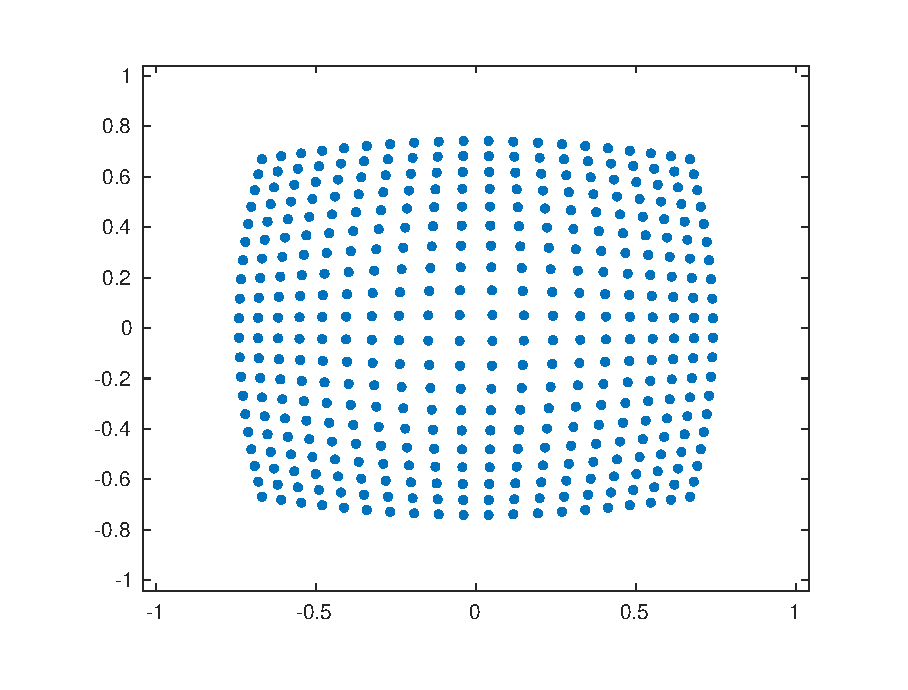
\includegraphics[width=7cm]{figs/post_distortion.eps}}
\caption{Barrel distortion applied to a rectangular grid, normalised to the range [-1,1]}
\label{barreldist}
\end{figure}

Pincushion distortion refers to the stretching of the image, particularly at the edges. It can be modelled with Brown's distortion model, the model and an example is given in section \ref{barSection}.  The inverse of pincushion distortion, barrel distortion, shown in figure \ref{barreldist}, can be applied to reverse the effects of pincushion distortion. The barrel distortion that the Oculus SDK\cite{oculus} applies results in a varying number of texels per pixel in our final image, a property will be explored in an extension.

Lens astigmatism is a property of the lenses used in most consumer HMDs. Because of the astigmatism, the image presented to the user is sharp in the center but becomes progressively blurrier as you look towards the edges as seen in figure \ref{blurred}. It can be corrected for by adding more lenses to the HMD, but this ends up being too expensive and bulky for consumer versions.

\begin{figure}
\centerline{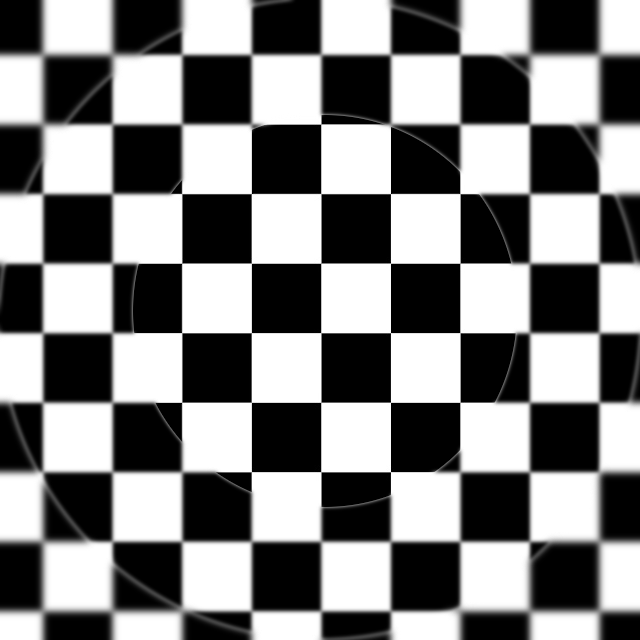
\includegraphics[width=5cm]{figs/blur.png}}
\caption{A depiction of lens astigmatism. The perceived image blurs as you move away from the sharp center.}
\label{blurred}
\end{figure}

This astigmatism property can be exploited by anti-aliasing only where the image is sharpest, in the center. Graphical artefacts at the edges should be blurred enough to be unnoticeable. It is this principle that I'll develop the following anti-aliasing approaches on top of.

\chapter{Preparation}

This chapter outlines any preparatory work that was done before implementation of the two anti-aliasing approaches.

\section{Previous Work}

This project was inspired by the Intel Research's 2015 publication: Using Astigmatism in Wide Angle HMDs to Improve Rendering \cite{Astigpap}. They exploited the astigmatism in an Oculus DK1 headset to decrease sampling at the edges of the image in a raytracer. They managed to improve the performance by a factor of $\approx 2.5$ in that raytracer.
Adjusting the sampling rate across the image in a raytracer is relatively straightforward. D. Pohl et Al used a \emph{sampling map} to achieve this. However, this may not be so easy or efficient in a rasterizer like OpenGL. In this project I take this idea of reducing sampling at image edges and apply it to a rasterizer. Rasterizers are a faster though less accurate rendering method - and, because of the intense timing constraints on Virtual Reality, are used significantly more in VR applications. 

\section{OpenGL}

The OpenGL API provides an interface to render 3D graphics. It's cross language, with native C bindings, well documented, and the most widely adopted open source graphics API. As a bonus it supports some efficient anti-aliasing standards.

Below I describe some OpenGL terminology that will be used lots later.

\begin{description}

\item\texttt{Framebuffer} \\
  A collection of buffers that can be used as the destination for rendering.

\item\texttt{Blitting} \\
  The process of moving image data between framebuffers.

\item\texttt{Front Buffer} \\
  The buffer containing the image that is presented on-screen now. This buffer is contained within the Default Framebuffer.

\item\texttt{Back Buffer} \\
  The buffer containing the image that will be presented on-screen in the next frame, is contained within the Default Framebuffer. 

\item\texttt{Primitive} \\
  An interpretive scheme used to determine what a stream of vertices represents when being rendered. For example \texttt{GL\_POINTS} causes each vertex to be interpreted as a point. Other primitive types include \texttt{GL\_TRIANGLES} and \texttt{GL\_LINES}
\item\texttt{Fragment} \\
  Collection of values produced by the rasterizer. A fragment represents a sample-sized segment of a rasterized primitive. These are processed by the fragment shader. 
\end{description}

\subsection{The OpenGL pipeline}

OpenGL provides a pipeline through which data about the rendered scene is processed and rasterized. A simplified view of it is presented here, given that some stages are optional or non-programmable.


\begin{figure}
\setlength{\unitlength}{0.8mm}-
\begin{center}
\begin{picture}(80,120)

\put(0,100){\framebox(80,10){Vertex Data}}
\put(0,80){\framebox(80,10){Vertex Shader}}
\put(0,60){\framebox(80,10){Geometry Shader}}
\put(0,40){\framebox(80,10){Primitive Assembly, Rasterization}}
\put(0,20){\framebox(80,10){Fragment Shader}}
\put(0,0){\framebox(80,10){Per Sample Operations}}



\put(40,20){\vector(0,-1){10}}
\put(40,40){\vector(0,-1){10}}
\put(40,60){\vector(0,-1){10}}
\put(40,80){\vector(0,-1){10}}
\put(40,100){\vector(0,-1){10}}

\end{picture}
\end{center}
\caption{A glimpse at the OpenGL rendering pipeline}
\label{latexpic2}
\end{figure}

Vertex data enters the pipeline, typically it has been uploaded to the GPU through a \texttt{Vertex Buffer Object}. Each vertex usually has associated data such as a colour, a normal vector, and texture coordinates.
The Vertex Shader is run for every vertex in the scene. In the typical case it transforms vertexes in 3d world space to window space coordinates. Vertex data from the previous scene is bound in through named variables.

The Geometry Shader is run for every primitive in the scene (in all of the implementations here I've simplified these to triangles as a general case). It is an unusual stage in that it can amplify geometry, outputting more primitives than it takes as input. This stage is optional, but it's used later on.

The Fragment shader is run for every fragment in the window space, it is typically used to perform lighting and texturing for the scene.

\section{Development}

Being relatively new to OpenGL I decided to build a toy renderer to teach myself the basics of the API.

This toy renderer proved invaluable to the success of the project, since I knew and understood the source code completely, I could implement and test an idea for optimization or an implementation strategy quickly. The toy renderer was implemented in C++.

To get an idea of how these implementations would fare in a larger, more computationally intensive renderer I decided to modify the demo provided with the Oculus SDK 5.0.1: OculusWorldDemo.
The codebase to this was in C++ and the rendering code was written to be extensible - allowing for different graphics APIs to implement higher level rendering calls. The OpenGL implementation was Open Source and under the Apache License.

An agile approach was taken when implementing the anti-aliasing methods, stories were broken up into small, manageable chunks. After these were implemented - extensions could be written up and implemented on top.
Unit tests were written for all new methods. However, where methods and classes were extended beyond Oculus' implementation, unit tests were not added due to the high degree of coupling within OculusWorldDemo and OpenGL and the extensive API mocking required. To make up for this, and to ensure correctness, runtime assertions were made on all branches and method calls.

\section{Software libraries}

The OculusVR SDK was used in the Demo to interface with the Oculus Rift DK2 HMD. An outdated version 0.5.0.1 was used being the last version to support Linux.
The SDK provided vector and matrix math modules, runtime assertions, and allowed barrel distortion and chromatic aberration to be performed.

GLFW was used for context creation in the toy renderer.
GLM was used for matrix math in the toy renderer.

\section{Programming Languages}

C++ was used in both the toy renderer and OculusWorldDemo. It integrates well with the OpenGL C bindings and has extensive compiler support allowing for performance to be maximised.

GLSL is the OpenGL C-like shader language that is run on the GPU. It was used to write the geometry shader in section \ref{optimisations} and the fragment shader in section \ref{blending}. It's syntax is very similar to C. Learning it was not particularly time-consuming.

\section{Development Tools}

\begin{itemize}
\item Sublime text was the editor used to write all the software here.

\item The C/C++ debugger \texttt{gdb} was used to debug both the toy renderer and OculusWorldDemo.

\item AMD's GPUPerfStudio was used to profile both OculusWorldDemo and the toy renderer.

\item \texttt{BuGLe} was used to debug the OpenGL calls in both the toy renderer and OculusWorldDemo.

\end{itemize}
\subsection{Version Control}

Git was used as a version control system due to its flexibility and my familiarity with it. Remote repositories were placed both on a separate hard-drive and Github. These remotes were updated on every commit. Commits were made after every development story was completed.

\subsection{Failsafes}

In the event of failure of my development machine, MCS machines were compatible and tested with the software I was using. Also two backups were made of all changes to the codebase, detailed above.

\chapter{Implementation}

This chapter describes the implementation of anti-aliasing techniques briefly outlined in Section \ref{vrdisplays}. I first give a brief introduction to OculusWorldDemo's structure - and then describe a general implementation strategy for two anti-aliasing techniques: Subscreen Multisampling, and Subscreen Supersampling. I also give an optimization to the latter that is available to OpenGL 4.0 and another that is available on some OpenGL ES implementations. 

Where source code has been modified, I will use the colour \textcolor{green}{green} to represent modifications I have made. However blocks of code that I have written entirely will follow the usual code formatting.

\section{OculusWorldDemo Structure}

Given that the implementation of two anti-aliasing techniques is built on top of Oculus' existing work, it was first necessary to understand a large portion of their codebase.
Here I give a brief overview of system components that will be modified and used later on. I also give a brief overview of Oculus' SDK before detailing components that were added and modified to OculusWorldDemo.

\begin{itemize}
\item OculusWorldDemoApp \\
  The class describing the application OculusWorldDemo, contains high level rendering instructions, calculation of HMD values, user input (Mouse, Keyboard), state initialization and more.

\item RenderDevice \\
  The module containing rendering state and methods, called by OculusWorldDemoApp. Provides several implementations of its methods in DirextX and OpenGL. Handles shader compilation, linking, GPU memory allocation for vertex \& texture data and more.

\end{itemize}
\section{The Render Loop}
At every frame, the Oculus SDK provides head-tracking information that must be used to maintain the appropriate user position and orientation in the program.

The bulk of rendering code is done within the OculusWorldDemoApp::OnIdle() method, which determines if and when a frame should be drawn, along with other bookkeeping.
For each frame the following must be done:

\begin{itemize}
  \item The SDK call \texttt{ovrHmd\_BeginFrame()} should be called to mark the beginning of the frame.
  \item Update head-tracking state.
  \item Draw the scene to some texture(s) $\tau$.
  \item Call \texttt{ovrHmd\_EndFrame($\tau$)}.
\end{itemize}

The Oculus SDK then takes $\tau$ and applies barrel distortion and chromatic aberration through a post-processing stage. 

\section{Barrel Distortion}\label{barSection}

A common model used to model barrel distortion is Brown's distortion model. 

\[
f(\vec p) = \frac{(\vec p)}{1-\alpha(\vec p)}
\]
Where $(\vec p)$ represents some point in the source image, and $p_i\in[-1,1]$. The constant $\alpha$ represents the amount of distortion applied to the image and is a property of the lens.


\begin{figure}[tbh]
\begin{center}
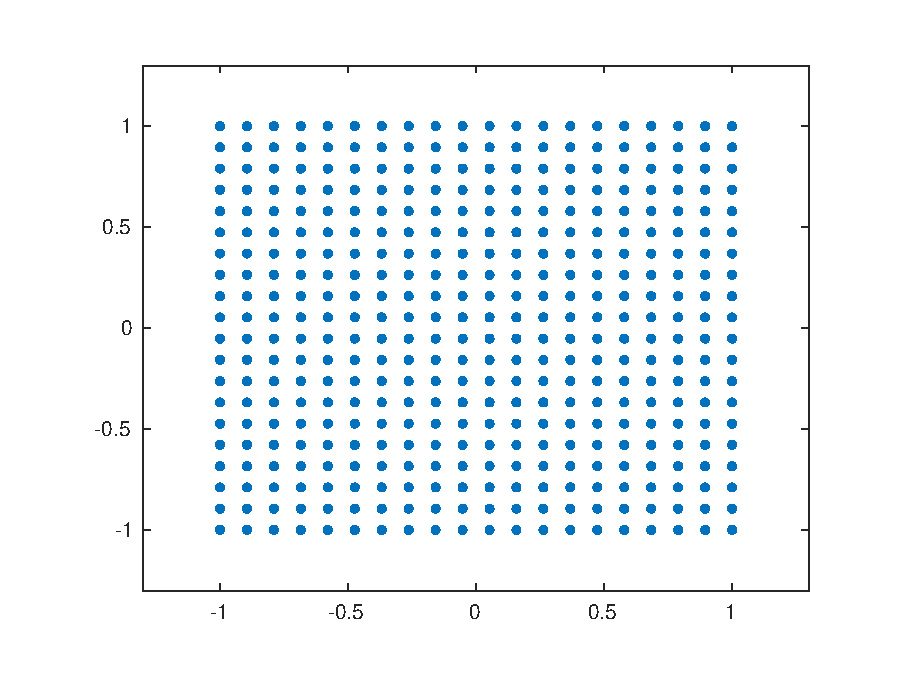
\includegraphics[width=6cm]{figs/pre_distortion.eps}
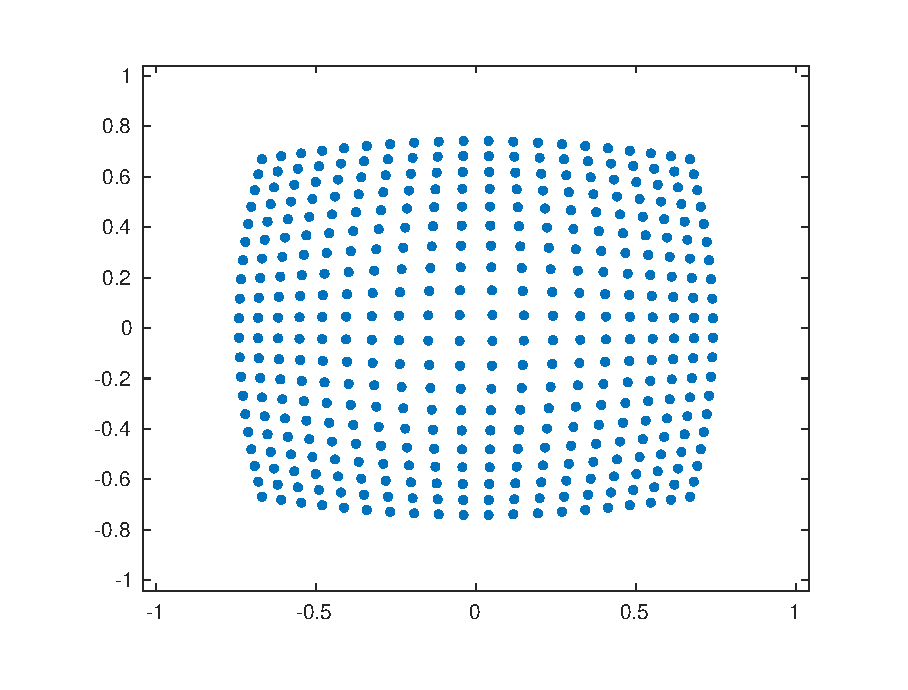
\includegraphics[width=6cm]{figs/post_distortion.eps}
\caption{Shows a regular pixel grid pre and post brown distortion, with $\alpha = 0.35 $.}
\label{epsfig1}
\end{center}
\end{figure}

The method used to combat pincushion distortion in VR has evolved over the past few years. Initially, barrel distortion was calculated per fragment as a post-processing step in the fragment shader. Later, the image provided to the post-processing step was used to texture a mesh whose vertices have the distortion applied, as can be seen in figure \ref {fig:meshgrid}. The latter approach is adopted by the Oculus SDK 5.0.1. Another approach, Vertex Displacement, involves distorting the scene into 'lens space'. It can be built into the rendering pipeline in the vertex shader, it removes the need for post-processing, but additionally requires the use of tessellation. \cite{vertexDisplacement}

\begin{figure}[tbh]
\begin{center}
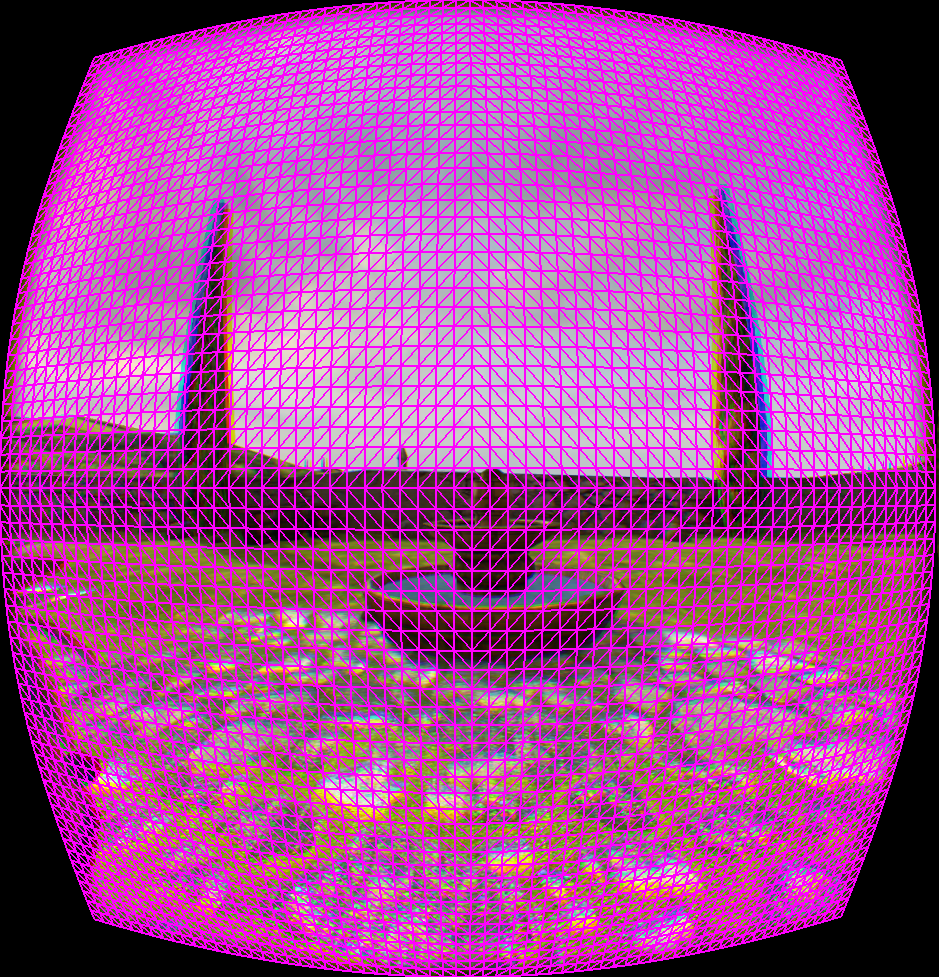
\includegraphics[width=6cm]{figs/barrelgrid.png}
\caption{Shows a render of OculusWorldDemo being used to texture a mesh, achieving barrel distortion.}
\label{fig:meshgrid}
\end{center}
\end{figure}


\section{Implementation overview} 

A high level implementation strategy is presented here. Each section will be detailed later on in the chapter.
To achieve Subscreen Antialiasing we can:

\begin{enumerate}
\item Specify two separate views. One for the low detail peripheral, and one for the low field of view, high detail center. Textures allocation and projections must be dealt with here.
\item Render to the two separate textures.
\item Finally, blend these textures onto the texture presented to the Oculus SDK. 
\end{enumerate}

Each of these steps can be generalised to handle both Subscreen Supersampling and Subscreen Multisampling. Section \ref{projections} handles step 1, section \ref{texturealloc} handles step 2, and section \ref{resolving} handles the final step.

\begin{figure}[tbh]
\begin{center}
\includegraphics[width=10cm]{figs/highlevelprocess.eps}
\caption{Shows a high level process of achieving Subscreen Antialiasing.}
\label{fig:meshgrid}
\end{center}
\end{figure}

\section{Projection Transformation} \label{projections}

An essential component to 3D graphics is the projection transformation. It takes as input 3D coordinates and maps them to 2D window coordinates.
Two types of projection must be dealt with in the implementation. 

\subsection{Orthographic projection}
The orthographic projection is a form of parallel projection, where all projection lines are parallel to the \texttt{lookAt} vector. 

\[
\begin{pmatrix}
\dfrac{2}{right-left} & 0 & 0 & -\dfrac{right+left}{right-left} \\
0 & \dfrac{2}{top-bottom} & 0 & -\dfrac{top+bottom}{right-left} \\
0 & 0 & \dfrac{2}{far-near} & -\dfrac{far + near}{far-near} \\
0 & 0 & 0 & 1
\end{pmatrix}
\]

This matrix is used to render two dimensional information at a required distance from the user. In OculusWorldDemo and others it is used to render UI components.
\subsection{Perspective projection}

The perspective projection is also used to render 3D scenes.
\[
\begin{pmatrix}
\dfrac{2*near}{right-left} & 0 & \dfrac{right + left}{right - left} & 0 \\
0 & \dfrac{2*near}{top-bottom} & \dfrac{top+bottom}{top-bottom} & 0 \\
0 & 0 & -\dfrac{far + near}{far-near} & -\dfrac{-2far*near}{far-near} \\
0 & 0 & -1 & 0
\end{pmatrix}
\]

To project onto a smaller portion of the screen it's necessary to specify alternate orthographic and perspective projection matrices that correspond to the smaller viewing frustum in the center of the screen. In OculusWorldDemo I specify new matrices: \texttt{OrthoProjectionSmall} and \texttt{OrthoProjection} corresponding to the center and peripheral view respectively. 

\subsection{Matrix Initialisation}\label{matrix}

The Oculus SDK will provide to the programmer the estimated field of view from the vector going from the eye to the center of the image. This information can be used to construct a frustum and projection matrix use in rendering.

\begin{figure}[tbh]
\centerline{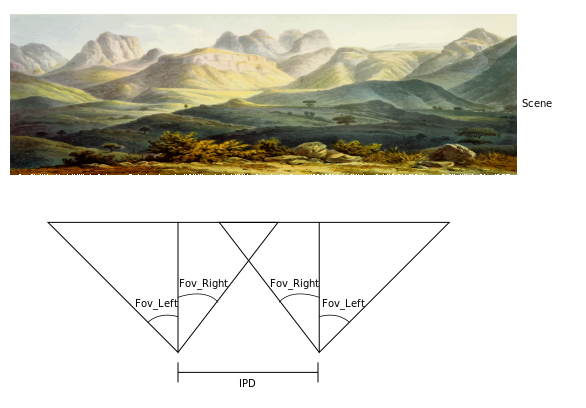
\includegraphics[scale=0.6]{figs/asymmetrical_fov.png}}
\caption{Shows the field of view for each eye. Not shown are the fov\_Up and fov\_Down parameters. IPD represents the Inter Pupillary Distance of the user - The distance between the center of each eye $\approx66mm$.}
\label{epsfig1}
\end{figure}

This information can be used to compute a matrix for both the full field of view and reduced, central field of view.

In the common case however, given a matrix \texttt{m} representing the projection for a full, symmetric field of view, the matrix for a smaller field of view can be computed with the following method.

\begin{blockcode}
Matrix4f centeredSmallMatrix(Matrix4f m, float ratio){
    Matrix4f rtn; 
    rtn = copyMatrix(m);
    rtn.M[0][0] *= ratio; //vertical FOV * 1/ratio
    rtn.M[1][1] *= ratio; //horizontal FOV * 1/ratio
    return rtn;
}
\end{blockcode}

The above returns a projection matrix whose near planes dimensions are $\frac{1}{\texttt{ratio}}$ of the input projection matrix's near plane. This small matrix will correspond to the smaller field of view whose render target will have higher quality anti-aliasing applied. 

\section{Allocating Textures}\label{texturealloc}

The framebuffer that is used must be complete before we begin rendering to it, so textures must be allocated and formatted properly beforehand. This section will describe texture allocation in OpenGL, and how the implementation in OculusWorldDemo was modified to permit the approach outlined before. 
 
The Oculus SDK provides a method \texttt{ovrHmd\_GetFovTextureSize()} that returns a reccomended texture size for a given Field of View and texel to pixel density at the center of the screen.

The process for allocating a framebuffer in OpenGL that contain render target textures that are $\frac{1}{r}$ the size of the destination texture is the same as normal framebuffer generation. Render target sizes must be divided by $r$, and implementations should take care of integer division here.

\section{Drawing the scene}

The perspective transformation is usually performed in the vertex shader stage, so the perspective transformation matrix must be linked up to this stage.
This matrix can be linked up to the vertex shader with the function \texttt{glUniformMatrix4fv()}.\\

The render method of each scene needs only to know which eye it is rendering to, and whether it is drawing to the center or the borders of the image. 
So the render method in OculusWorldDemoApp was modified to include the perspective projection matrix of the portion of the scene it is drawing to.

\begin{blockcode}[commandchars=\\\{\}]
void OculusWorldDemoApp::RenderEyeView(ovrEyeType eye,
                                       \color{green}Matrix4f * projection,
                                       \color{green}Matrix4f * orthoProj)
\end{blockcode}

You can then bind the correct projection matrices inside this method with a call to \texttt{glUniformMatrix4fv()}
Nothing else needs altering in the draw call for this implementation.

\subsection{Modifying The Render Loop}

Before beginning to render to each view with corresponding framebuffer $F$, OpenGL state needs to be set up. Therefore for each framebuffer $F$ the following steps are needed inside of the render loop. 4 Framebuffers can be used to achieve a stereoscopic view with subscreen multi-sampling or super-sampling.

\begin{enumerate}

\item Bind $F$ to the draw framebuffer.
\item Set the viewport to the resolution of $F$.
\item Draw the scene onto $F$.

\end{enumerate}

As I will describe later on, this process can be handled on the GPU side with the use of the geometry shader, freeing up the CPU and reducing the number of draw calls to a half.

\section{MultiSample Resolve}\label{resolving}

With a multi-sampled or super-sampled texture along with a single sampled border texture, a resolve from the multi-sampled or super-sampled texture to the destination buffer needs to be performed to merge the two together before presenting on-screen. This can be achieved with a blit operation or blending in a post-processing stage.
The function below takes as arguments a multi-sampled or super-sampled texture along with an output texture. It then resolves the samples from the source texture to the target texture. The method doesn't care whether the source texture is multi-sampled or super-sampled, these cases will be identified from the source texture's flags.

\begin{smallcode}[commandchars=\\\{\}, numbers=left]
void RenderDevice::ResolveMsaa(OVR::Render::Texture* msaaTex, OVR::Render::Texture* outputTex, float ratio)
\{
    bool isMsaaTarget = msaaTex->GetSamples() > 1;
    glBindFramebuffer( GL_READ_FRAMEBUFFER, MsaaFbo);
    glFramebufferTexture2D( GL_READ_FRAMEBUFFER, GL_COLOR_ATTACHMENT0,
                            isMsaaTarget ? GL_TEXTURE_2D_MULTISAMPLE : GL_TEXTURE_2D,
                            ((Texture*)msaaTex)->TexId, 0);
    glFramebufferRenderbuffer(GL_READ_FRAMEBUFFER, GL_DEPTH_ATTACHMENT, GL_RENDERBUFFER, 0);
    OVR_ASSERT(glCheckFramebufferStatus(GL_READ_FRAMEBUFFER) == GL_FRAMEBUFFER_COMPLETE);

    glBindFramebuffer( GL_DRAW_FRAMEBUFFER, CurrentFbo );
    glFramebufferTexture2D(GL_DRAW_FRAMEBUFFER, GL_COLOR_ATTACHMENT0, GL_TEXTURE_2D, ((Texture*)outputTex)->TexId, 0);
    glFramebufferRenderbuffer(GL_DRAW_FRAMEBUFFER, GL_DEPTH_ATTACHMENT, GL_RENDERBUFFER, 0);

    OVR_ASSERT(glCheckFramebufferStatus(GL_DRAW_FRAMEBUFFER) == GL_FRAMEBUFFER_COMPLETE);

\color{green}    int off_x = (outputTex->GetWidth() - outputTex->GetWidth()/ratio)/2; //Offset from bottom left of the target texture. 
\color{green}    int off_y = (outputTex->GetHeight() - outputTex->GetHeight()/ratio)/2; // ditto for height
\color{green}    glBlitFramebuffer( 0, 0, msaaTex->GetWidth(), msaaTex->GetHeight(), off_x, off_y,
\color{green}                             off_x + outputTex->GetWidth()/ ratio,
\color{green}                             off_y + outputTex->GetHeight()/ ratio,
\color{green}                             GL_COLOR_BUFFER_BIT, GL_LINEAR);

    glBindFramebuffer( GL_FRAMEBUFFER, 0 );  
    GLint err = glGetError();
    OVR_ASSERT_AND_UNUSED(!err, err);
\}
\end{smallcode}

The method needs to set up the OpenGL state machine for the \texttt{glBlitFramebuffer} on line 21. First a multi-sampled framebuffer is set up to be read in line 2. Next we associate this framebuffer with \texttt{msaaTex} in lines 3-4. 
We then set up the destination texture in its own framebuffer, and set the GL state to draw to this buffer in the blit in lines 11-13.

Note that assertions are made to check for framebuffer completeness. An incomplete framebuffer cannot be drawn to.

Lines 19-24 implement the last stage of the downsampling method given in Y. It's enough to only blit the color buffer and do a linear downsample. 

The GL\_LINEAR filter will perform a supersample resolve by taking a weighted linear combination of the destination texels nearest neighbors in the source texture. Given that the source textures texels are equally spaced, this linear filter implements the average given in \ref{supersampling}.

If the input texture is multisampled, and if the source and destination rectangles are the same size, OpenGL will perform a multisample resolve onto the destination framebuffer in hardware.

\section{OpenGL optimisations} \label{optimisations}

As a summary of the implementation so far, each frame has to be rendered in the following way:

\begin{itemize}
  \item Set the viewport and projection matrix for the inner field of view.
  \item Render a multisampled or supersampled view of the scene onto some render target.
  \item Set the viewport and projection matrix for the outer field of view.
  \item Render the outer field of view.
\end{itemize}
The approach given has two main disadvantages:

For each frame:
\begin{itemize}
  \item The entire scene must be traversed on each draw call - That's twice for each eye.
  \item Many near identical draw calls are made, where only user perspective and position changes.
\end{itemize}

This situation can be improved twofold by taking advantage of the geometry shader.

\section{Amplifying Geometry}

Instead of submitting a draw call for each viewport, it's possible to provide projection and view information to the geometry shader, which can decide which projection matrix to apply to which view. It can then, for each primitive it receives, send one to each specified view in a single draw call. This can be used to render to the two views needed to achieve Subscreen Supersampling, or as explained in section \ref{stereoScopic}, can be used to render two stereoscopic images in one draw call.

\subsection{The Geometry Shader}

First, we need to effectively disable the vertex shader. It can simply be redefined to pass through all its input data onwards towards the geometry shader.
Then, the geometry shader can handle the perspective projection.

\begin{figure}[tbh]
\centerline{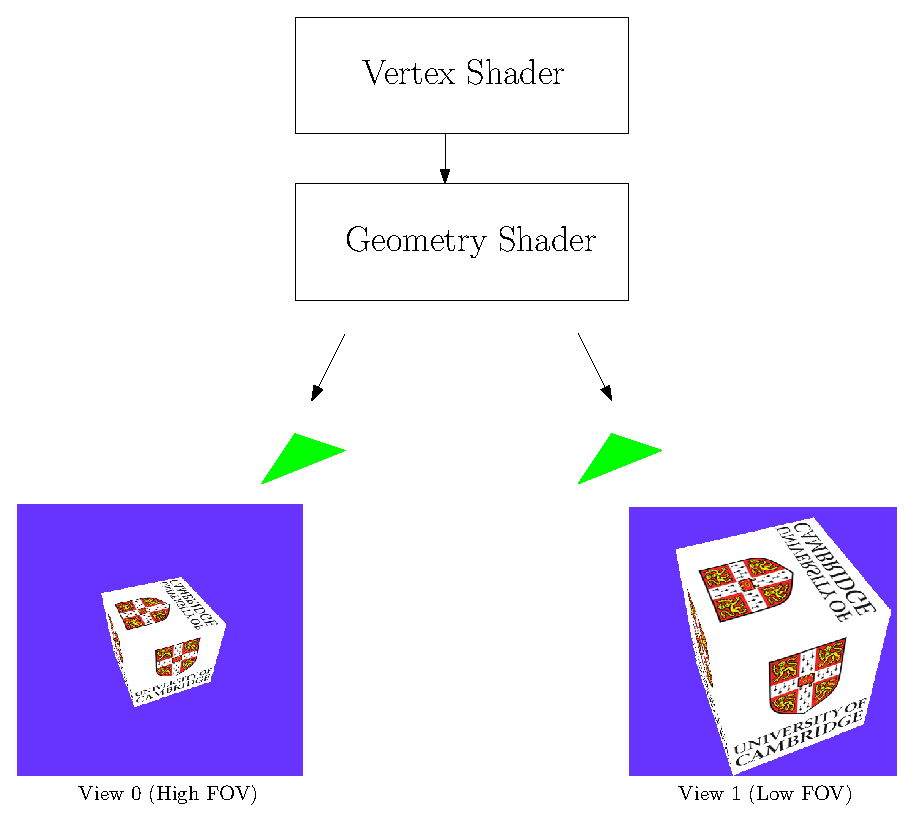
\includegraphics[scale=0.6]{figs/geoshader.eps}}
\caption{Shows the high level process of rendering to two resolutions with one draw call}
\label{epsfig1}
\end{figure}

It's possible to either simultaneously render to separate layers of a layered texture, or simultaneously render to two separate viewports within the same, large texture. I use the latter approach for simplicity, and to allow the two textures to be easily resized, a property that will be useful when tuning the extension. I also assume 4 samples per pixel in this implementation, though it's not difficult to apply this to higher or lower levels of sampling. 

This optimisation requires the OpenGL extension \texttt{ARB\_viewport\_array} \cite{arbViewport} though it is ubiquitous across modern implementations.

First, we must specify our viewports' dimensions:

\begin{blockcode}
float v[] = {0, 0, mWidth, mHeight,
             mWidth, 0, mWidth*2, mHeight};
glViewportArrayv(0, 2, v); //Specify a viewport array, of length 2
\end{blockcode} 

The above initialises a viewport array such that the first viewport occupies the left half of the texture, and the second the right half of the screen. Viewport 0 will have a high field of view rendered to it, while Viewport 1 will have a low field of view, representing the area we will supersample.\\

Next the geometry shader must be enabled and compiled. Below, I give a snippet of the relevant geometry shader code.

\begin{blockcode}
  layout(triangles) in;
  layout(triangle_strip, max_vertices=6) out;
  ...
  for (i=0; i<2; i++){
    currentProj = i==0 ? proj : projSmall; //select currentProj based on i

    fColour = vColour[0];
    fTexCoord = vTexCoord[0];
    gl_Position = currentProj*view*model*gl_in[0].gl_Position;
    EmitVertex();
    gl_ViewportIndex = i;
  ...
  EndPrimitive();
\end{blockcode}

As required by the geometry shader the input and output primitive type are specified. This same code can be specialized for other primitive types, but triangles are shown here being the general case.
Then we can loop over the viewports, emitting a primitive at each.

Line 5 selects the projection matrix based on the looping variable \texttt{i}. Then, colour, texture and normal information are passed on to the fragment shader for use in lighting and texturing. Finally the position of the vertex is calculated by the standard Model, View, Perspective transformation, along with the index of the viewport it will be sent to. This snippet is applied to all vertices in the primitive.

The resulting wide framebuffer can then be resolved in the same way given in section \ref{resolving}. The right half of the screen can be blitted onto the left half.
Alternatively, you could perform a downsample in the barrel distortion shader, though this alternative wasn't implemented.  

\section{Extension 1: Non-uniform Texel Density}

In section \ref{barSection} I introduced barrel distortion, and its implementation in modern Virtual Reality SDKs. Briefly, a mesh whose vertexes have been distorted according to some model is textured with a rectangular view of the scene. This texture, whose smallest elements I refer to as \emph{texels}, has texel values that might never contribute to the final colour presented on the display. This can be explained by use of figure \ref{fig:barreldensity1}.

\begin{figure}[tbh]
\begin{centering}
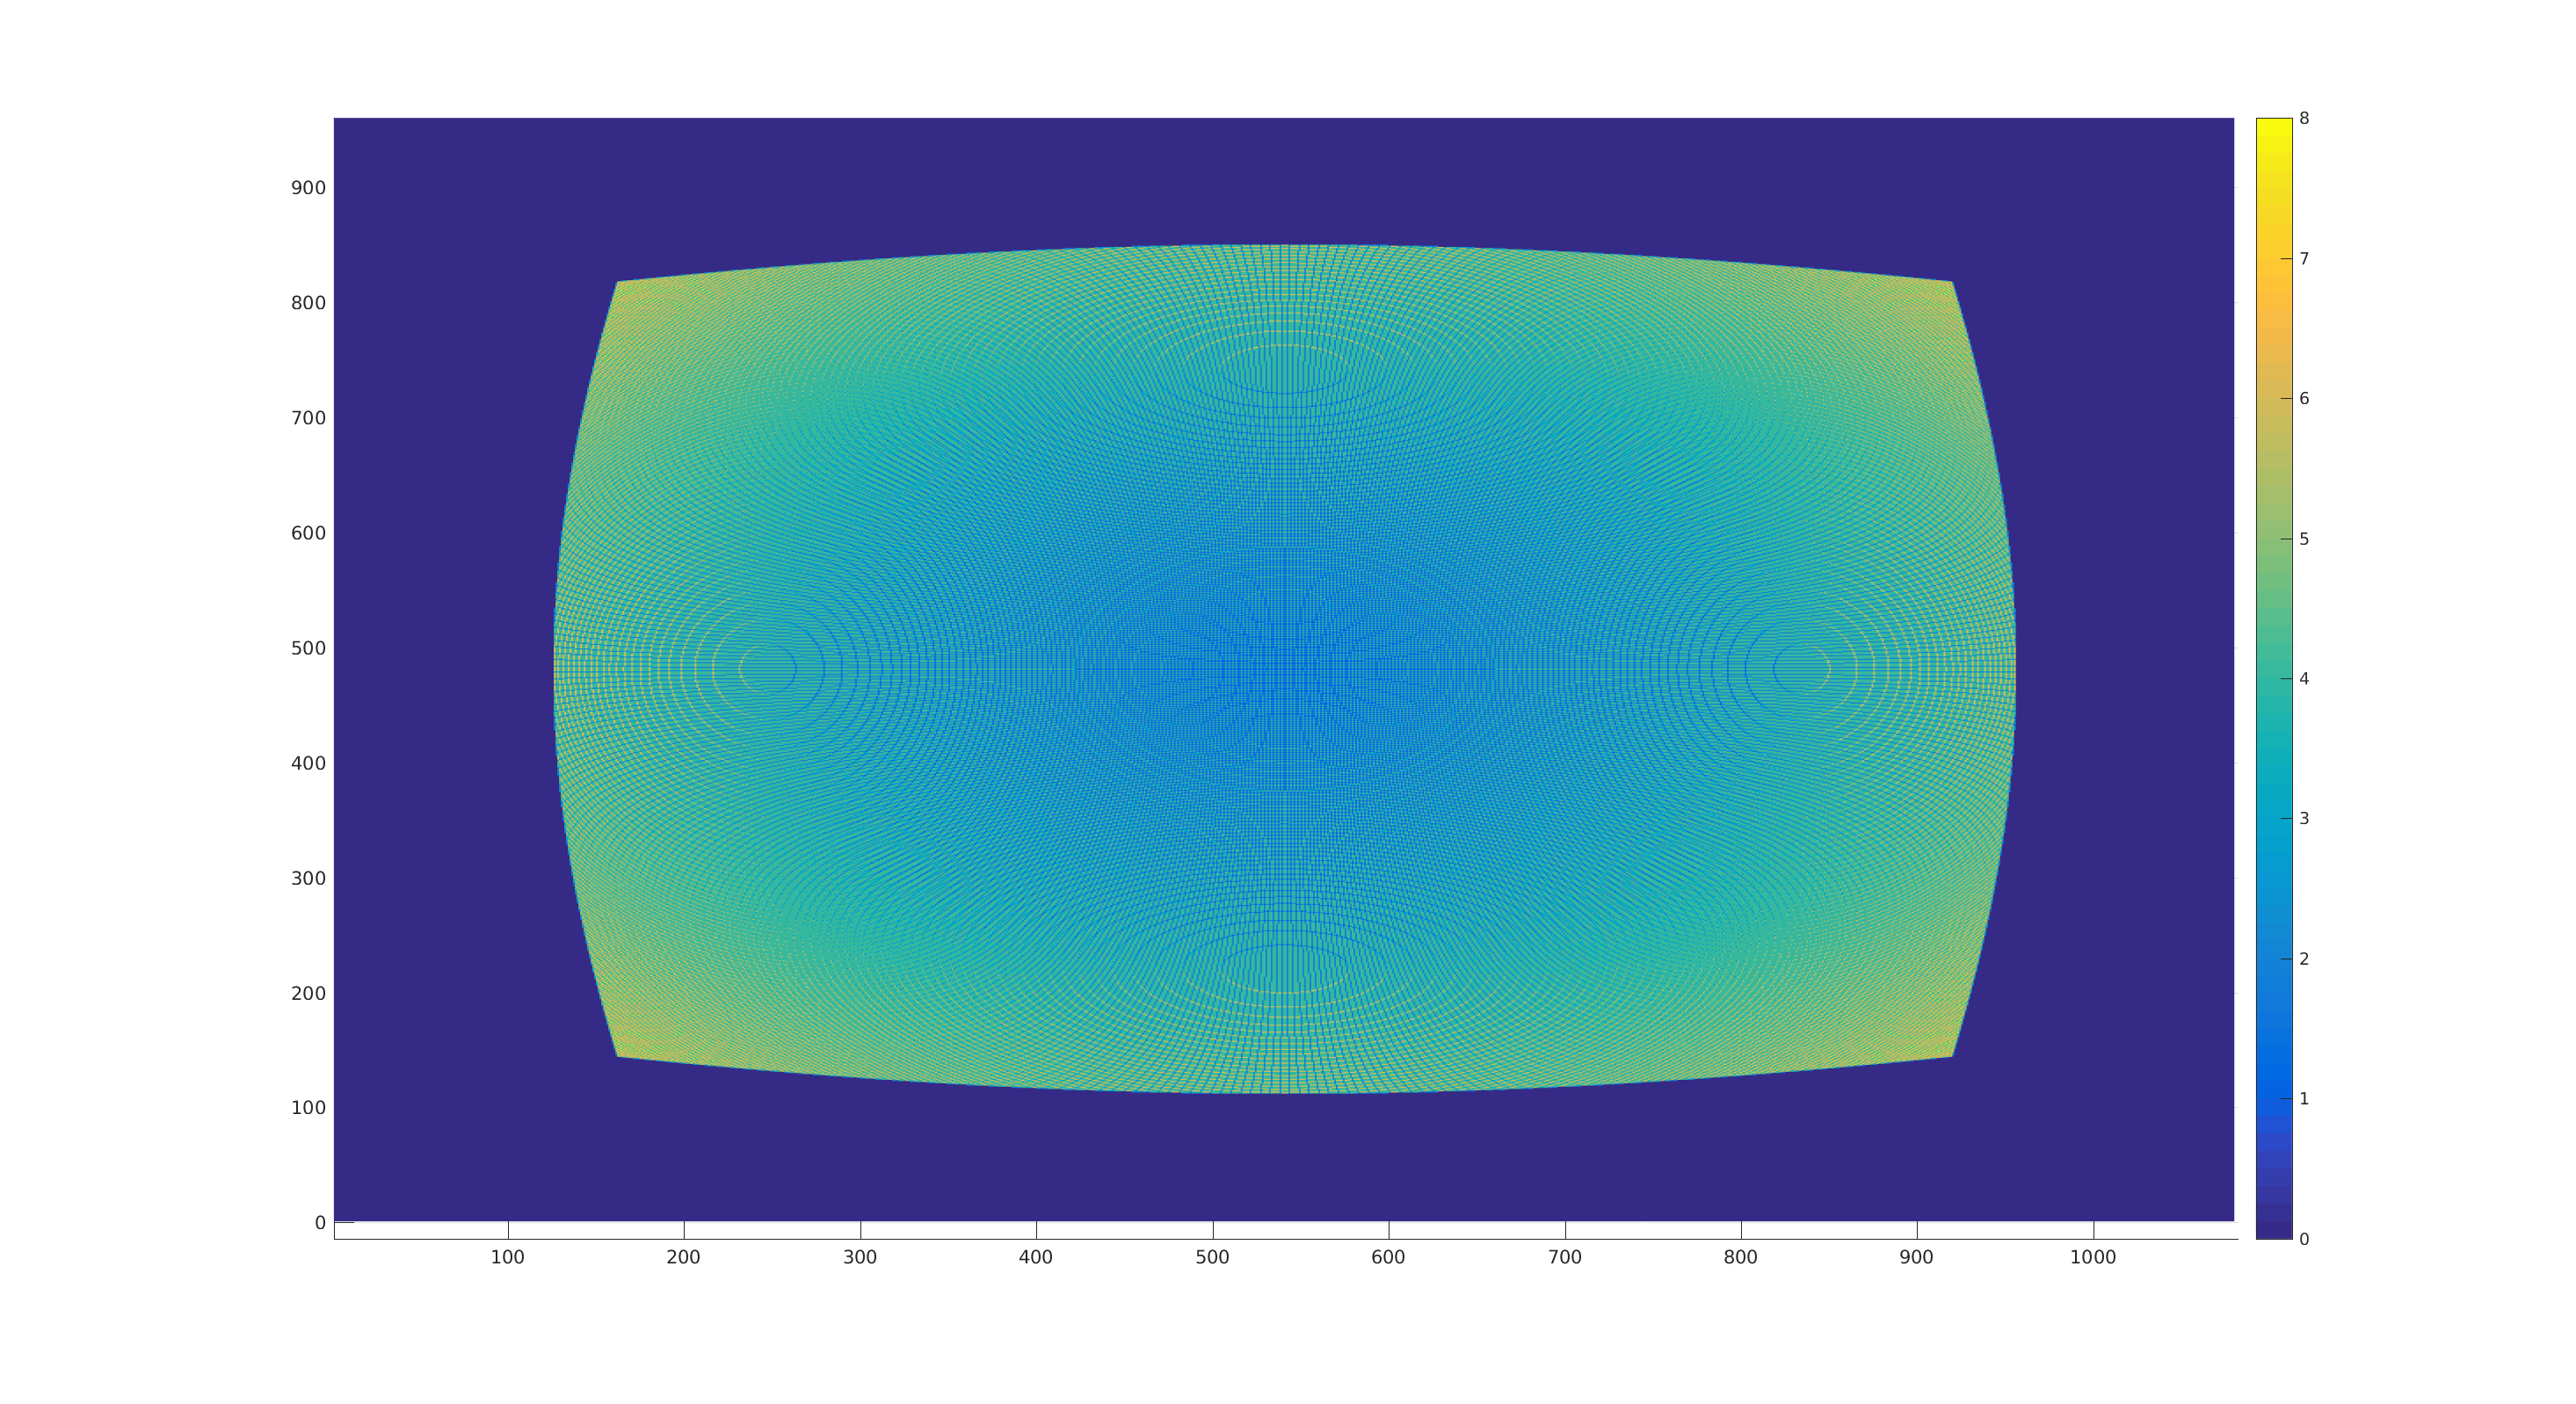
\includegraphics[width=12cm]{figs/oculus_pixel_density.eps}
\label{epsfig1}
 
\caption{Shows the texel per pixel density across a barrel distorted image at the recommended Oculus DK2 texture size.}
\label{fig:barreldensity1}
\end{centering}
\end{figure}

Texel to pixel density is lowest at the center of the image and highest in the edges. If a bilinear texture lookup is used, some texels won't contribute to the colour on the mesh, wasting fragment processing. Ideally we would like a 1-1 mapping from a projection space texel and a barrel distortion space pixel. This can be achieved with the use of \emph{vertex displacement} \cite{vertexDisplacement}, though this approach has its own drawbacks, requiring geometry tessellation. Another approach that can help us approach the desired 1-1 mapping is by projecting the scene onto cascaded frusta. Projection onto cascaded frusta describes the process of projecting the scene onto a series of textures with a series of frusta, and each frustum in the series occupying an increasing field of view.
This process also describes exactly that implemented for subscreen anti-aliasing, with the additional requirement that the wide field of view texture be downsized, to prevent redundant fragments being processed. We've also implemented a geometry shader to allow simultaneous rendering of two fields of view with a single draw call. 

It's possible to render below a single texel per pixel threshold near the image edge, exploiting astigmatism in the lens. My implementation renders to textures of the same size, which should reduce fragment shading by approximately half. Note that the resulting image goes slightly below the 1 texel per pixel threshold in the peripheral. However, it's possible to increase to achieve at least 1-1 mapping by fine tuning the resolution of the two textures and still make savings in fragment processing.

\subsection{Blending the two textures}\label{blending}

A blit operation between the low and high resolution texture might be wasteful, given that the rendertarget is not anti-aliased, and would require an upscale of the lower resolution texture, wasting GPU memory and forcing an unnecessary blit operation. So a better method would be to blend the two textures in a post-processing stage. Given that barrel distortion is performed as post-processing, we can choose whether to sample from the high Field of View texture or low Field of View texture based on whichever has the highest sampling frequency at a point on the mesh. To do this, access to the render buffer texture can be modified using the following method:

\begin{figure}[tbh]
\centerline{\includegraphics[width=8cm]{figs/textureblend.eps}}
\caption{Shows the texture coordinates for the low field of view texture given on the outer rectangle. The low field of view texture can then be sampled correctly in the fragment shader.}
\label{fig:texblend}
\end{figure}

\begin{enumerate}
\item For the rectangle used for texturing onto, we can provide two texture coordinates, one for the low field of view image, and one for the high field of view. An example for my implementation is given in figure \ref{fig:texblend}. This is done to avoid unnecessary texture coordinate arithmetic inside of the fragment shader.
\item Sample both the low field of view texture and high field of view in the fragment shader of post-processing using the respective varying texture coordinates.
\begin{blockcode}
	vec4 lowFovSample = texture(texFramebufferLowFov, lowFovTexCoord);
	vec4 highFovSample = texture(texFramebufferHighFov, highFovTexCoord);
\end{blockcode}

\item Based on the low field of view texture coordinates, choose either the low field of view, or high field of view sample.

\begin{blockcode}	
	outColour = greaterThan(vec2(0.0,0.0), lowFovTextureCoord) && 
				lessThan(lowFovTextureCoord, vec2(1.0,1.0)) 
				? lowFovSample : highFovSample;

	//selects the lowFovSample if it's within 
	//the correct texture bounds (0,0), (1,1) 
\end{blockcode}
\end{enumerate}

The texture coordinates for the post-processing step were taken from the ARM Mali VR Documentation \cite{armDeveloper}, though the fragment shader was written by myself. 

\section{Stereoscopic rendering}

The situation described in section \ref{optimisations} also describes a typical stereoscopic rendering loop. That is, we need to duplicate draw calls between eyes even though only uniform matrices (Model, View, Projection) differ between the draw calls. It's possible use the exact same code to render both eye views of a stereoscopic image in one call. Instead of providing Model, View, and Projection (MVP) matrices that correspond to a low field of view and a high field of view as before, we can instead provide two MVP matrices that correspond to each eye. All that remains is attaching them to the shader program with a call to \texttt{glUniformMatrix4fv()}. With this optimization and the optimization given in section \ref{optimisations} it's possible to achieve a fourfold reduction in the number of draw calls and scene traversals than in the na\"ive implementation.

\section{Limitations}

While some optimization was allowed for Subscreen Supersampling through the use of the geometry shader, hardware support is needed to perform Subscreen Multisampling efficiently.
An API extension that allowed for simultaneous drawing to two targets could help to perform Subscreen Multisampling much more efficiently.
Multi-projection hardware is available for some GPU vendors \cite{multiResShading}, and this would give a considerable speedup to most of the techniques given here. 

\section{Future Hardware Support}

The disadvantage of the geometry shader approach to multi-resolution shading is the incurred cost of invoking the optional geometry shader stage.
Two extensions to OpenGL have been proposed by Oculus, \texttt{OVR\_MULTIEW} \cite{OVRmultiview}, and \texttt{OVR\_MULTIVIEW2} \cite{OVRmultiview2}. These extensions will allow multiple elements of a 2D texture array to be rendered to simultaneously. Allowing rendering both to the high resolution central image and lower resolution peripheral in one call, without the need for invoking the geometry shader and without intrusive modifications to the vertex shader. The only implementations of these extensions are in GLES currently - perhaps because of the vendor specific multi-projection hardware in modern GPUs.

Regardless, a brief explanation of multi-resolution rendering using \texttt{OVR\_MULTIVIEW} will be given here.

\begin{itemize}

\item First we need to set up a layered texture.

\item Then, a framebuffer must be generated, and the layered texture attached to it. This can be done using the new function \texttt{glFramebufferTextureMultiviewOVR}
\begin{footcode}
glFramebufferTextureMultiviewOVR(GL_DRAW_FRAMEBUFFER, GL_COLOR_ATTACHMENT0,
				 frameBufferTextureId, 0, 0, 2); // attach layered texture
\end{footcode}
\item Then, we can generate depth buffers for each layer, and attach them to the framebuffer:
\begin{footcode}
glFramebufferTextureMultiviewOVR(GL_DRAW_FRAMEBUFFER, GL_DEPTH_ATTACHMENT,
				 frameBufferDepthTextureId, 0, 0, 2); //attach layered depth
\end{footcode}
\item Finally, an assertion on framebuffer completeness should be made.
\begin{footcode}
//assert framebuffer is complete
OVR_ASSERT(glCheckFramebufferStatus(GL_DRAW_FRAMEBUFFER) == GL_FRAMEBUFFER_COMPLETE);
\end{footcode}

Then, in a manner similar to selecting a projection matrix based on the viewport ID in section \ref{optimisations}, a projection can be selected based on the variable \texttt{gl\_ViewID\_OVR} in the vertex shader like so.

\begin{footcode}
currentProj = gl_ViewID_OVR == 0 ? proj : projSmall; //select currentProj based on gl_ViewID 
\end{footcode}

\end{itemize}

The two textures can be blended in post-processing by the same method given in section \ref{resolving}

\chapter{Evaluation}

In this chapter I assess the objective image quality across all techniques developed. I also describe a user study carried out to asses the subjective image quality across techniques. Finally I give a variety of performance metrics to determine the performance across the techniques in a platform independent setting.

\section{Objective Assessment}

While a user study performs provides a robust assessment of image quality across different approaches, Computational metrics for objective image quality assessment can be essential. The performance of the system determines how quickly the image responds to stimulus which can help reduce simulation sickness in the user. Given that implementations of graphics APIs differ dramatically, along with hardware implementations, measuring a framerate directly on a particular machine cannot be the best indicator of performance as a whole. Though the render time per frame of different approaches are given, it should be understood that performance can vary dramatically across different hardware vendors, graphics APIs and their implementations, and rendering programs. Given this, a range of other information is given to best represent the anti-aliasing approaches and given some more meaningful insight into their execution. Information such as: triangle count, fragment and vertex shader invocations, API calls, GPU usage, CPU usage, along with some interpretation of this in a platform independent setting. Profiling information was gathered using the tool AMD GPUPerfStudio.

\section{API calls}

A reduction in the number of API calls we send to the GPU can contribute to better performance of the system. Every API call needs to be send to the GPU and validated, taking hundreds to thousands of instructions.

\begin{center}
\begin{tabular}{l|c|r}
Technique   & No. Draw Calls \\ 
\hline
No anti-aliasing      & 402 \\
Fullscreen Multisampling     & 402 \\
Subscreen Multisampling    &  802  \\
Fullscreen Supersampling      &  402   \\
Subscreen Supersampling    &  403  \\
\end{tabular}
\end{center}

Subscreen Multisampling could not be optimized in the same way as Subscreen Supersampling due to the OpenGL constraint that Complete Framebuffers' Layers must have the same number of samples. Therefore it was necessary to render the scene twice, explaining why it has twice the number of draw calls.

Because we were able to simultaneously draw to two textures in Subscreen Supersampling, it has the same number of draw calls as its fullscreen counterpart bar one. This extra call is present because the blending of the two images in this implementation was performed via an extra blit operation.

\section{Fragment shader invocations}

Fragment shader invocations generally increase linearly with the size of image. If our application bottleneck is at the fragment shader stage, we will reap performance benefits by shading less fragments.

\begin{figure}[tbh]

 
\begin{subfigure}{0.5\textwidth}
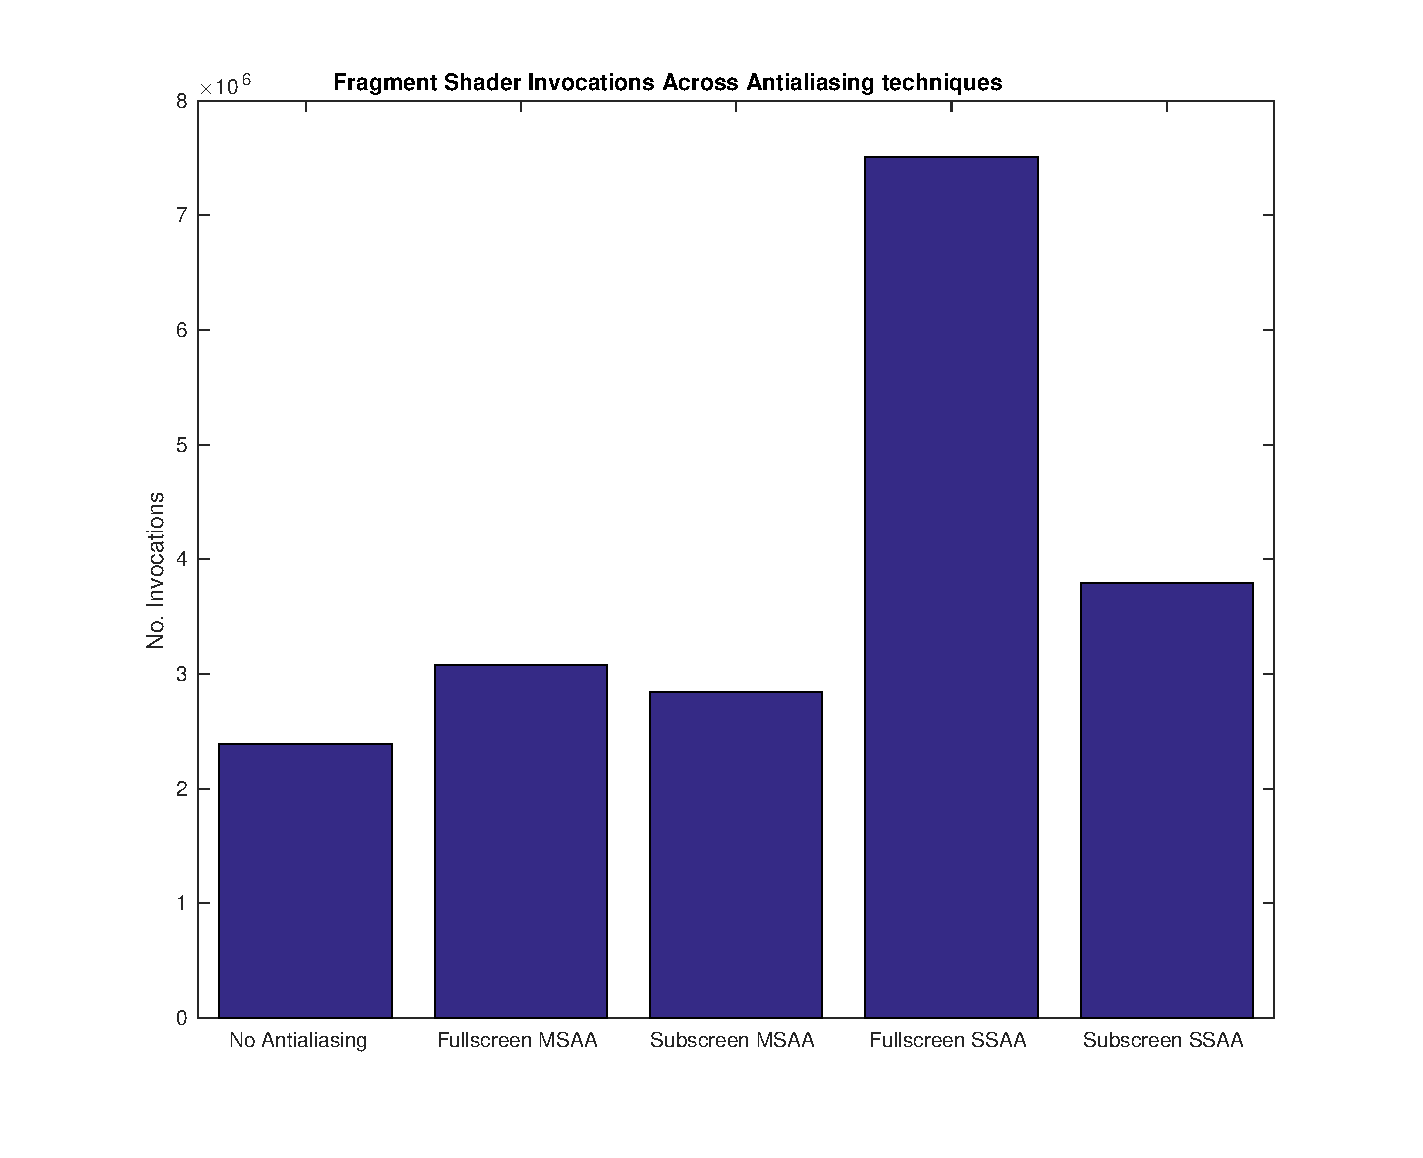
\includegraphics[height=7cm]{figs/fsInvocations.eps}
\end{subfigure}
\qquad
\begin{tabular}{l|c}
Technique   & No. Invocations \\ 
\hline
No anti-aliasing      & 2.3872e+06 \\
Fullscreen Multisampling     & 3.0753e+06 \\
Subscreen Multisampling    &  2.8465e+06  \\
Fullscreen Supersampling      &  7.5106e+06   \\
Subscreen Supersampling    &  3.7955e+06  \\
\end{tabular}
 
\caption{Shows the number fragment shader invocations across the different techniques.}
\end{figure}

As expected, significantly fewer fragments are shaded in subscreen analogues of fullscreen anti-aliasing techniques. In this instance Subscreen Multisampling shades 7.6\% fewer fragments, while Subscreen Supersampling shades 49.5\% fewer fragments. This is as expected, and fulfills the main success criterion of the project.

\clearpage

\section{Fragment Shader Timing}

A measurement representing the cumulative time spent processing fragments on the GPU is given below.

\begin{figure}[tbh]

 
\begin{subfigure}{0.5\textwidth}
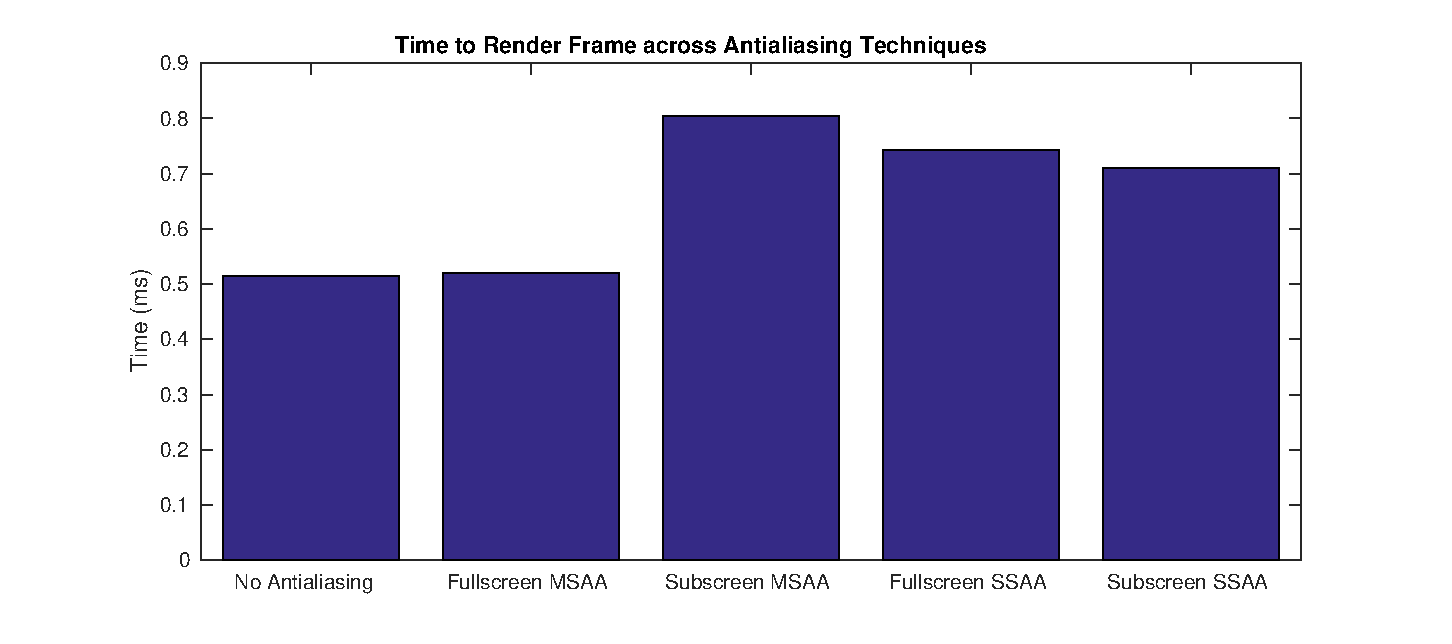
\includegraphics[width=1.2\linewidth]{figs/timeToRenderFrame.eps}
\end{subfigure}
\qquad
\begin{tabular}{l|c}
Technique   & Time (ms) \\ 
\hline
No anti-aliasing      & 0.30362 \\
Fullscreen Multisampling     & 0.30426 \\
Subscreen Multisampling    &  0.35263  \\
Fullscreen Supersampling      &  0.52043   \\
Subscreen Supersampling    &  0.34764  \\
\end{tabular}
 
\caption{Shows the time taken to process fragments across the techniques.}
\end{figure}

Surprisingly, less time is spent shading fragments in Subscreen Supersampling than in Subscreen Multisampling even though the former invokes the same shader code roughly 1 million times more. This can be attributed to the parallelization of draw calls in Subscreen Supersampling, whereas Subscreen Multisampling is forced to make double the number of API calls sequentially. It could also be down to the GPU being better able schedule fragment shaders, hide memory latency, and exploit caches more fully where all invocations are made available to the GPU in one batch. This result shows that the optimization made in section \ref{optimisations} makes a considerable improvement in the time processing fragments per frame, again fulfilling a success criterion of the project. \\

As expected, Subscreen Supersampling also outperforms its fullscreen counterpart, achieving a 33.3\% speedup in the Fragment Shader stage. 

\section{Geometry Processing}

A disadvantage of rendering multiple views is the cost of processing additional geometry. This is necessary hit that was justified by the following:

\begin{itemize}
\item Vertex processing tends to be simple and fast, typically only involving simple arithmetic operations.
\item The number of vertex shader invocations are vastly outnumbered by fragment shader invocations. 
\item Fragment shading tends to be more complex, requiring texture lookups, and lighting calculations.
\end{itemize}

A table detailing time spent processing geometry is given below. Note that only Subscreen Supersampling made use of the geometry shader to process geometry instead of the vertex shader, hence its apparent speedup in the vertex shader stage.  

\begin{tabular}{l|b{2.8cm}|b{3.5cm}|r}
Technique   & Vertex Shader Time (ms) & Geometry Shader Time (ms) & Total (ms) \\ 
\hline
No anti-aliasing      & 0.13772 & 0 & 0.13772 \\
Fullscreen Multisampling     & 0.13515 & 0 & 0.13515 \\
Subscreen Multisampling    &  0.24633 & 0 & 0.24633 \\
Fullscreen Supersampling      & 0.13788 & 0 & 0.13788 \\
Subscreen Supersampling    & 0.057913  & 0.23841 & 0.296323 \\
\end{tabular} \\

As expected, more time is spent processing geometry in both Subscreen Multisampling and Subscreen Supersampling. Slightly less time is spent performing 'useful work' in Subscreen Supersampling and Subscreen Multisampling. However, because the vertex shader cannot be disabled under OpenGL, time is spent on this stage even though the shader used in subscreen supersampling passes through all its inputs to its outputs without modification.  

\clearpage
\section{Removal of artefacts}\label{removeArtefacts}
By capturing views of a scene using different rendering techniques and subtracting them, we can observe artefacts that were present in the scene before and after anti-aliasing was applied. The image differences below have been thresholded, to make artefacts that have been removed more visible. 

\subsection{Subscreen Supersampling}

\begin{figure}
\begin{subfigure}{0.5\textwidth}
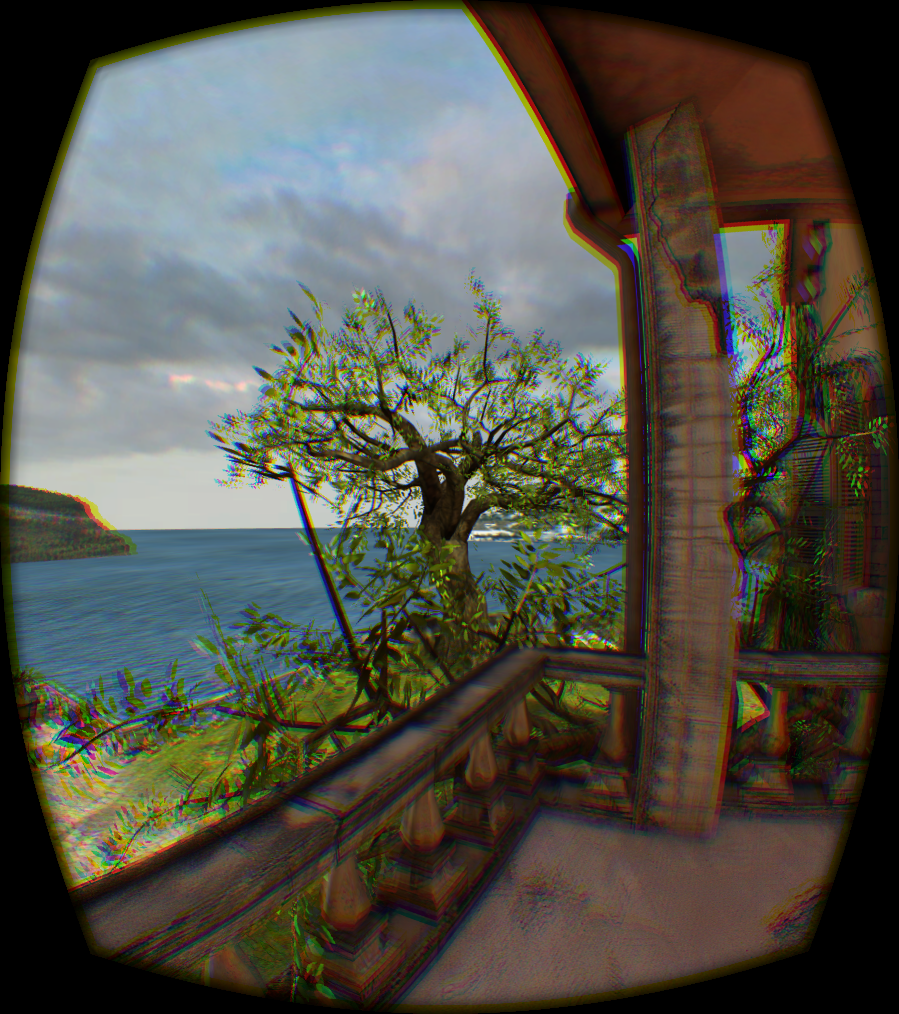
\includegraphics[width=0.9\linewidth]{figs/tree_msaa.png}
\caption{The original Scene}
\label{fig:subim2}
\end{subfigure}
\begin{subfigure}{0.5\textwidth}
\centerline{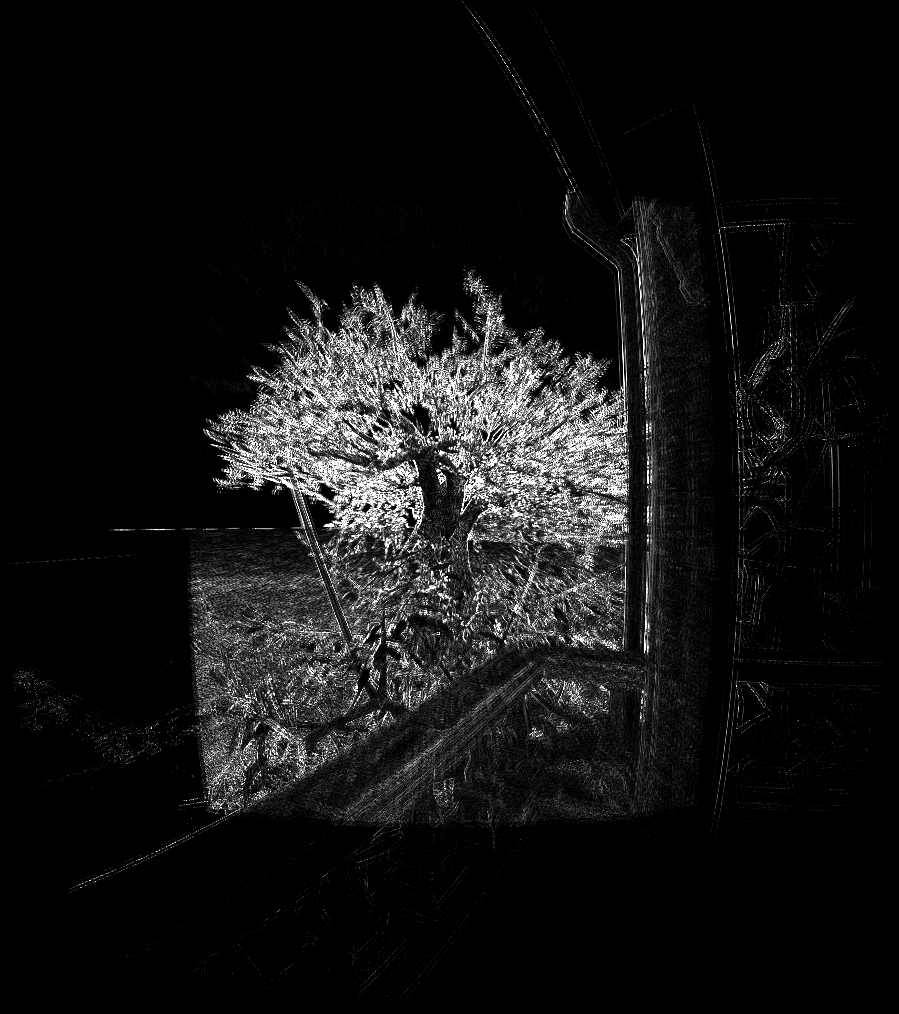
\includegraphics[width=0.9\linewidth]{figs/difftree.png}}
\caption{Fullscreen MSAA - Subscreen SSAA}
\label{ssaatree}
\end{subfigure}
 
\caption{Image of the tree scene showing the thresholded difference between Subscreen SSAA and Subscreen MSAA}
\label{fig:supersample}
\end{figure}

Using Supersampled Anti-aliasing, we can see in figure \ref{fig:supersample} texture filtering has improved. While multisampling only removes artefacts at polygon boundaries. Tree leaves inside of polygons are represented using alpha channel. Supersampling will ameliorate artefacts due to alpha testing, whereas multisampling cannot, hence the large difference between supersampling and multisampling in this scene.

\clearpage

\subsection{Subscreen Multisampling}

\begin{figure}[tbh]

\begin{subfigure}{0.5\textwidth}
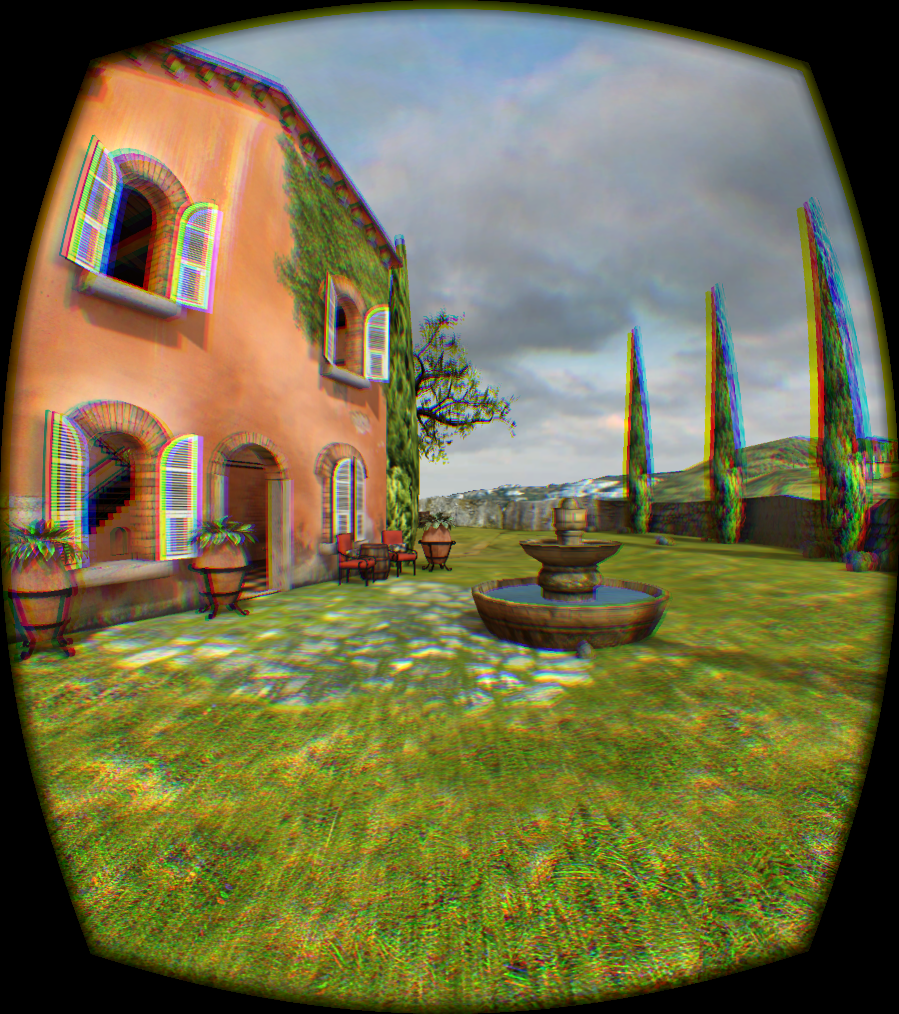
\includegraphics[width=0.9\linewidth, height=5cm]{figs/noantialiasing.png}
\caption{The original Scene}
\label{fig:subim2}
\end{subfigure}
\begin{subfigure}{0.5\textwidth}
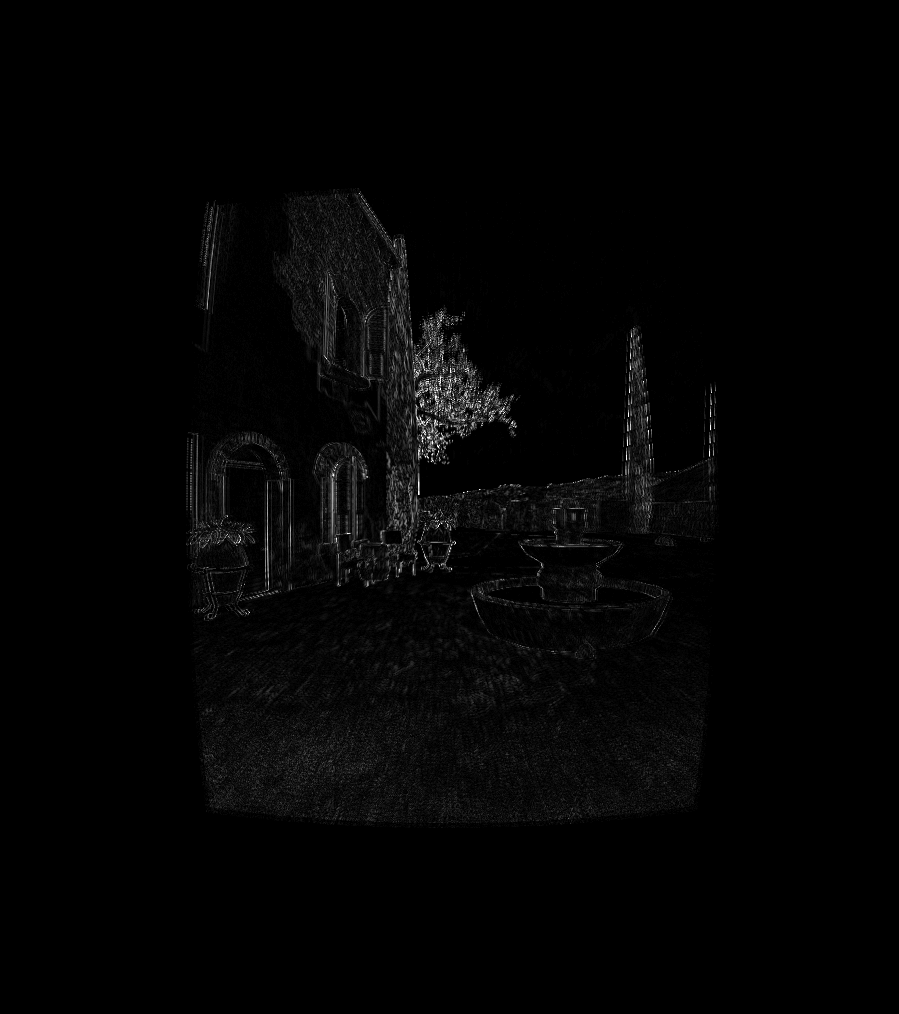
\includegraphics[width=0.9\linewidth, height=5cm]{figs/fullscreenminussubscreenmsaa.png} 
\caption{Fullscreen MSAA - Subscreen MSAA}
\label{fig:subim1}
\end{subfigure}
 
\caption{Highlights aliasing that is removed from both Subscreen MSAA and Fullscreen MSAA}
\label{fig:multisample}
\end{figure}

Subscreen MSAA works as expected here in figure \ref{fig:multisample}. Artefacts at polygon edges do not differ between fullscreen and subscreen. Interestingly, there is a minute difference in texturing between the two approaches. An explanation for this is a small, sub-pixel jitter applied to the projection matrix for the central area of the screen, thanks to reduced precision in transforming matrices in section \ref{matrix}.

\section{Subjective Assessment}
A user study was performed to asses the subjective quality across the techniques implemented. Section \ref{studySetup} describes the experiment, and section \ref{studyResults} describes its results.

\section{User Study Setup}\label{studySetup}

Subjects were given 3 different scenes to observe, with head-tracking enabled, across 4 different anti-aliasing techniques. They were: Fullscreen multisampling (4x), No anti-aliasing, Subscreen multisampling (4x), Subscreen supersampling (2x). The latter two being implemented by myself. Fullscreen Multisampling is the reference image - it is expected that this will provide the best image quality, and therefore comparisons will be made in reference to it.

Test subjects were presented with two images in succession, and asked to choose the one with better image quality, though the interpretation of a better quality image was left to the subject. All permutations of image comparison were presented to users. Each comparison was repeated three times in a (pseudo) random order. Each experiment took around 20 minutes with a total of 18 comparisons per scene.

The three scenes shown were:

\begin{enumerate}
\item A scene of green, untextured blocks, moving in a horizontal circle around the user.

\item A scene of a courtyard, including downsampled textures and complex geometry.

\item A scene from a balcony, facing a tree with alpha testing to implement leaves.
\end{enumerate}

All participants were made aware of their right to stop the experiment at any time, and approval was obtained from the Computer Laboratory Ethics Committee. 

\section{User study results}\label{studyResults}

To determine the difference of each technique with respect to a reference image (Fullscreen Multisampling), I use the Just-Objectionable-Difference (JOD) metric. A stimulus is 1 JOD from a reference stimulus if 75\% of users can tell the difference between them. I use the same method as Adhikarla, Vamsi Kiran, et al \cite{rafalPaper}. The tools used to calculate the JOD and the respective error were developed by my supervisor Rafal Mantiuk, and are available to use under the MIT License \cite{pwcomp}. 

\begin{figure}[tbh]
\centerline{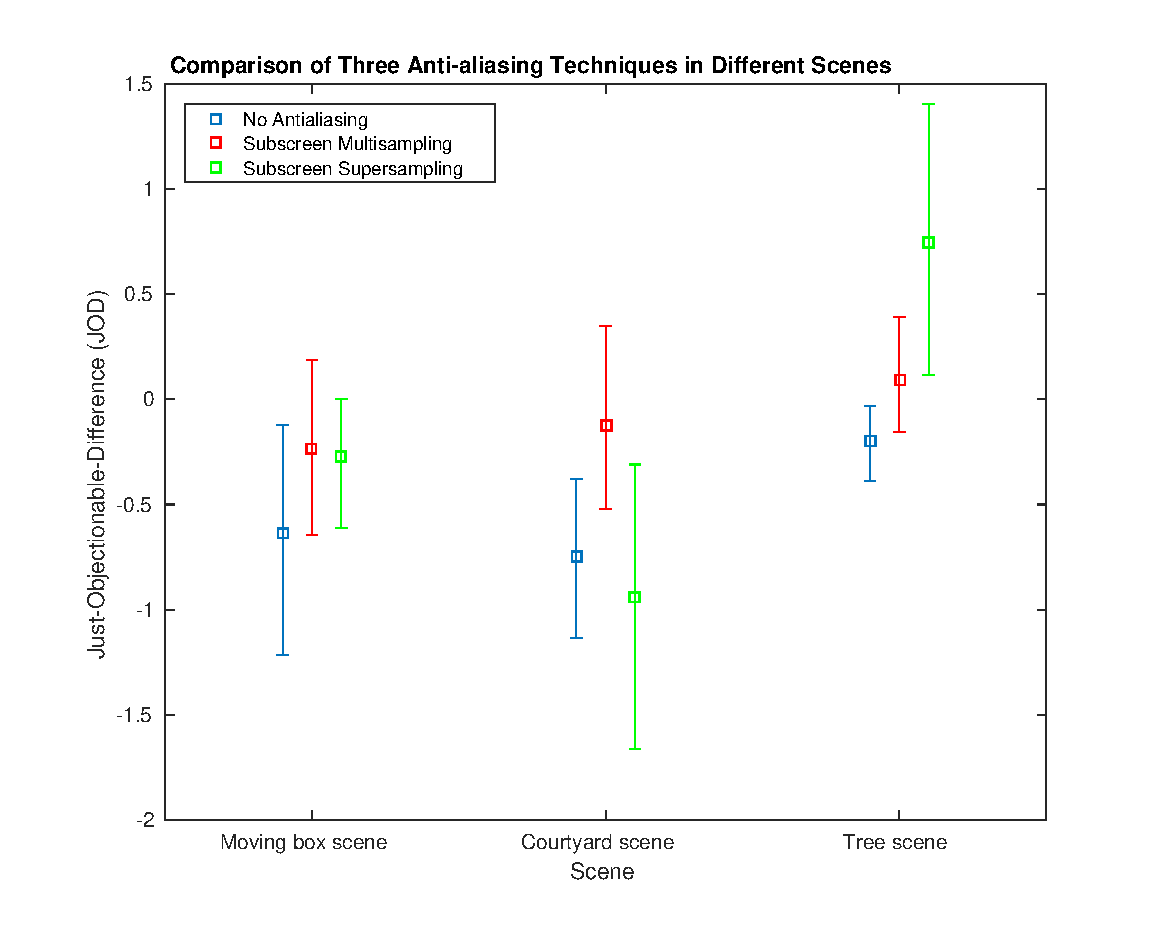
\includegraphics[width=14cm]{figs/jod.eps}}
\caption{Shows the Just-Objectionable-Difference(JOD) of three anti-aliasing techniques from a reference image of Fullscreen Multisampling. Greater JOD implies greater image quality to the reference.}
\label{fig:jod}
\end{figure}

Subscreen Supersampling was largely indistinguishable from its fullscreen counterpart with a very small JOD across all scenes, this could be because of the astigmatism of the headmounted display lenses or because fixation was more likely to reside in the centre of the view. This result was expected and helps to fulfill one success criterion of the project. 

No anti-aliasing performed generally worse than all other methods as expected. Although it outperformed Subscreen Supersampling in the courtyard scene. This might be because the difference in texture sampling between the centre and edges of the image were noticeable and jarring in this scene.

However Subscreen Supersampling performed best at the scene of the tree, with spatial artefacts owing to alpha testing being ameliorated only by supersampling, as explained in section \ref{removeArtefacts}.

Error in the results can be attributed to a few things: The small sample size, this experiment was performed on 10 subjects. Subtle differences between techniques makes the decision for the user harder, and increased error. 
In retrospect, given that Subscreen Supersampling outperformed the reference in the tree scene, a higher quality reference image should have been chosen. Were I to run the experiment again, I would choose fullscreen supersampling as a reference image. I might also allow subjects to switch between the two compared techniques at will before deciding on their preference, given that some artefacts are quite subtle.

The indistinguishability of subscreen multisampling and fullscreen multisampling is the most promising result from this user study, however.

\clearpage

\section{Extension 1 Evaluation}

Because of the barrel distortion applied in post-processing Oculus recommends rendering at a resolution \%40 larger than the display resolution to achieve an acceptable texel density in the center of the image.
A large problem facing the traditional barrel distortion applied in post-processing is a non-uniform texel density across the image. Furthermore, texel density is highest at the extremities, where gaze is less likely to be fixed and lens astigmatism will have the greatest impact. 

\begin{figure}[tbh]

\begin{subfigure}{0.5\textwidth}
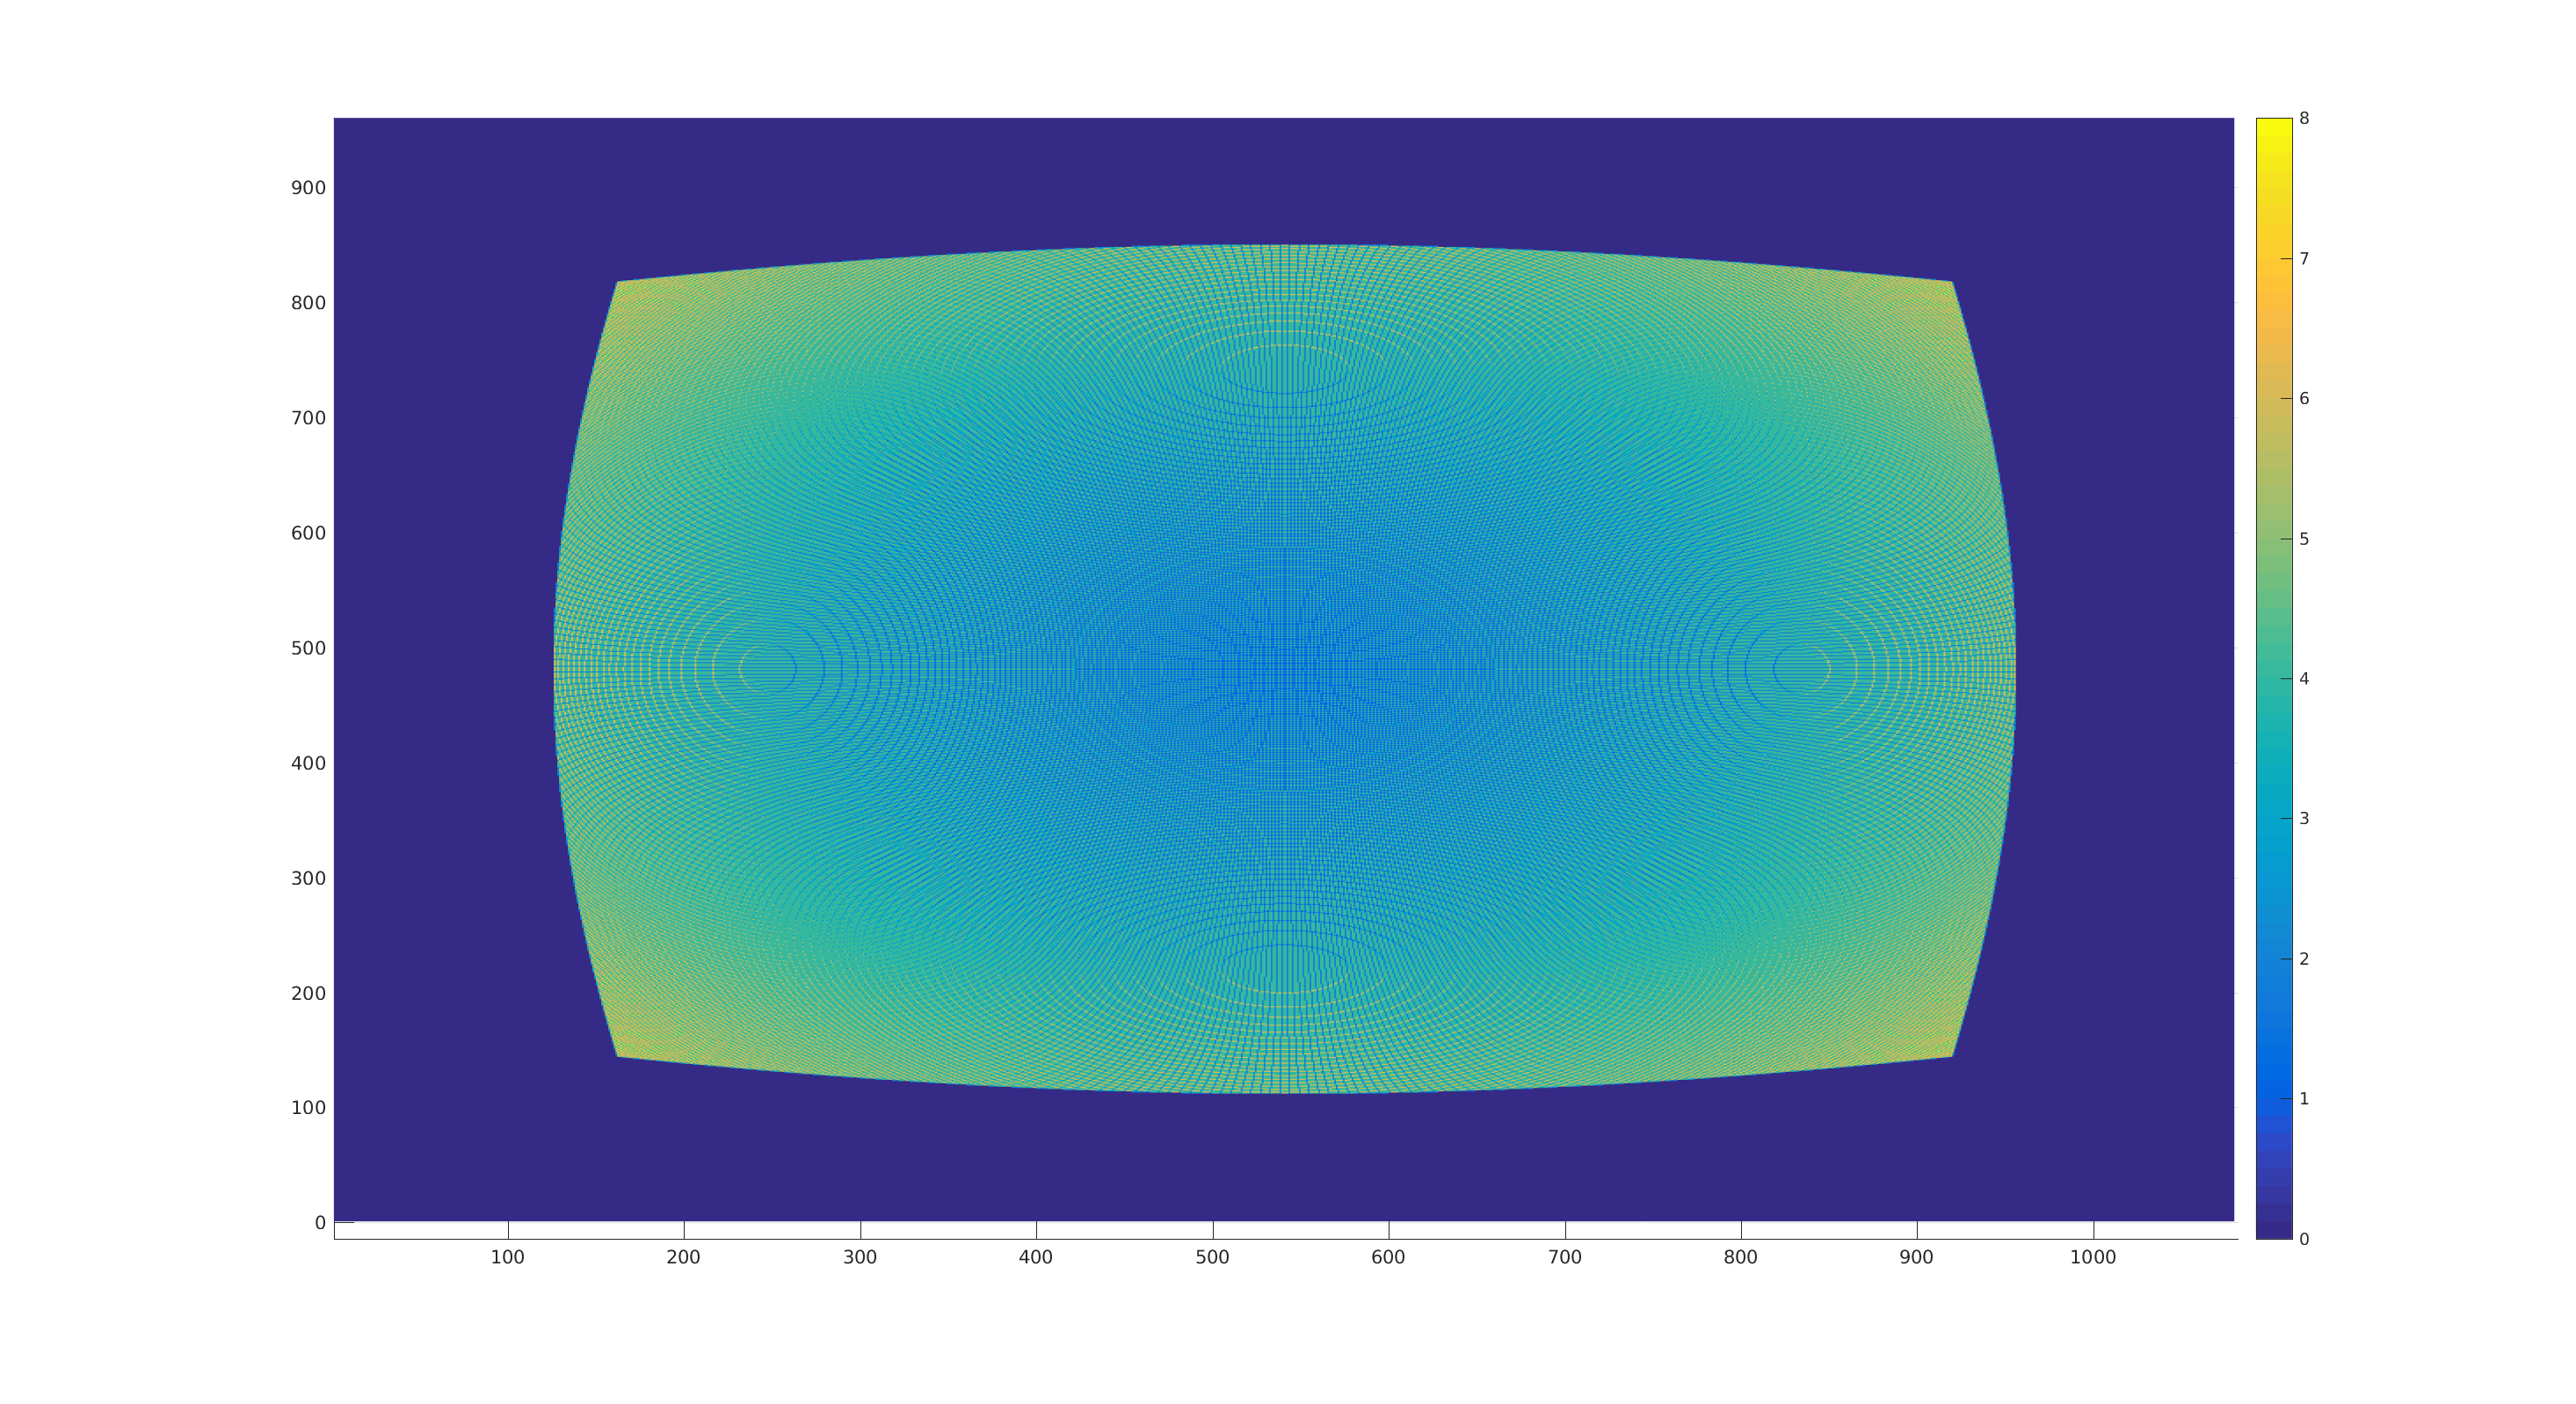
\includegraphics[width=1.2\linewidth]{figs/oculus_pixel_density.eps}
\caption{Original texel density}
\label{epsfig1}
\end{subfigure}
\begin{subfigure}{0.5\textwidth}
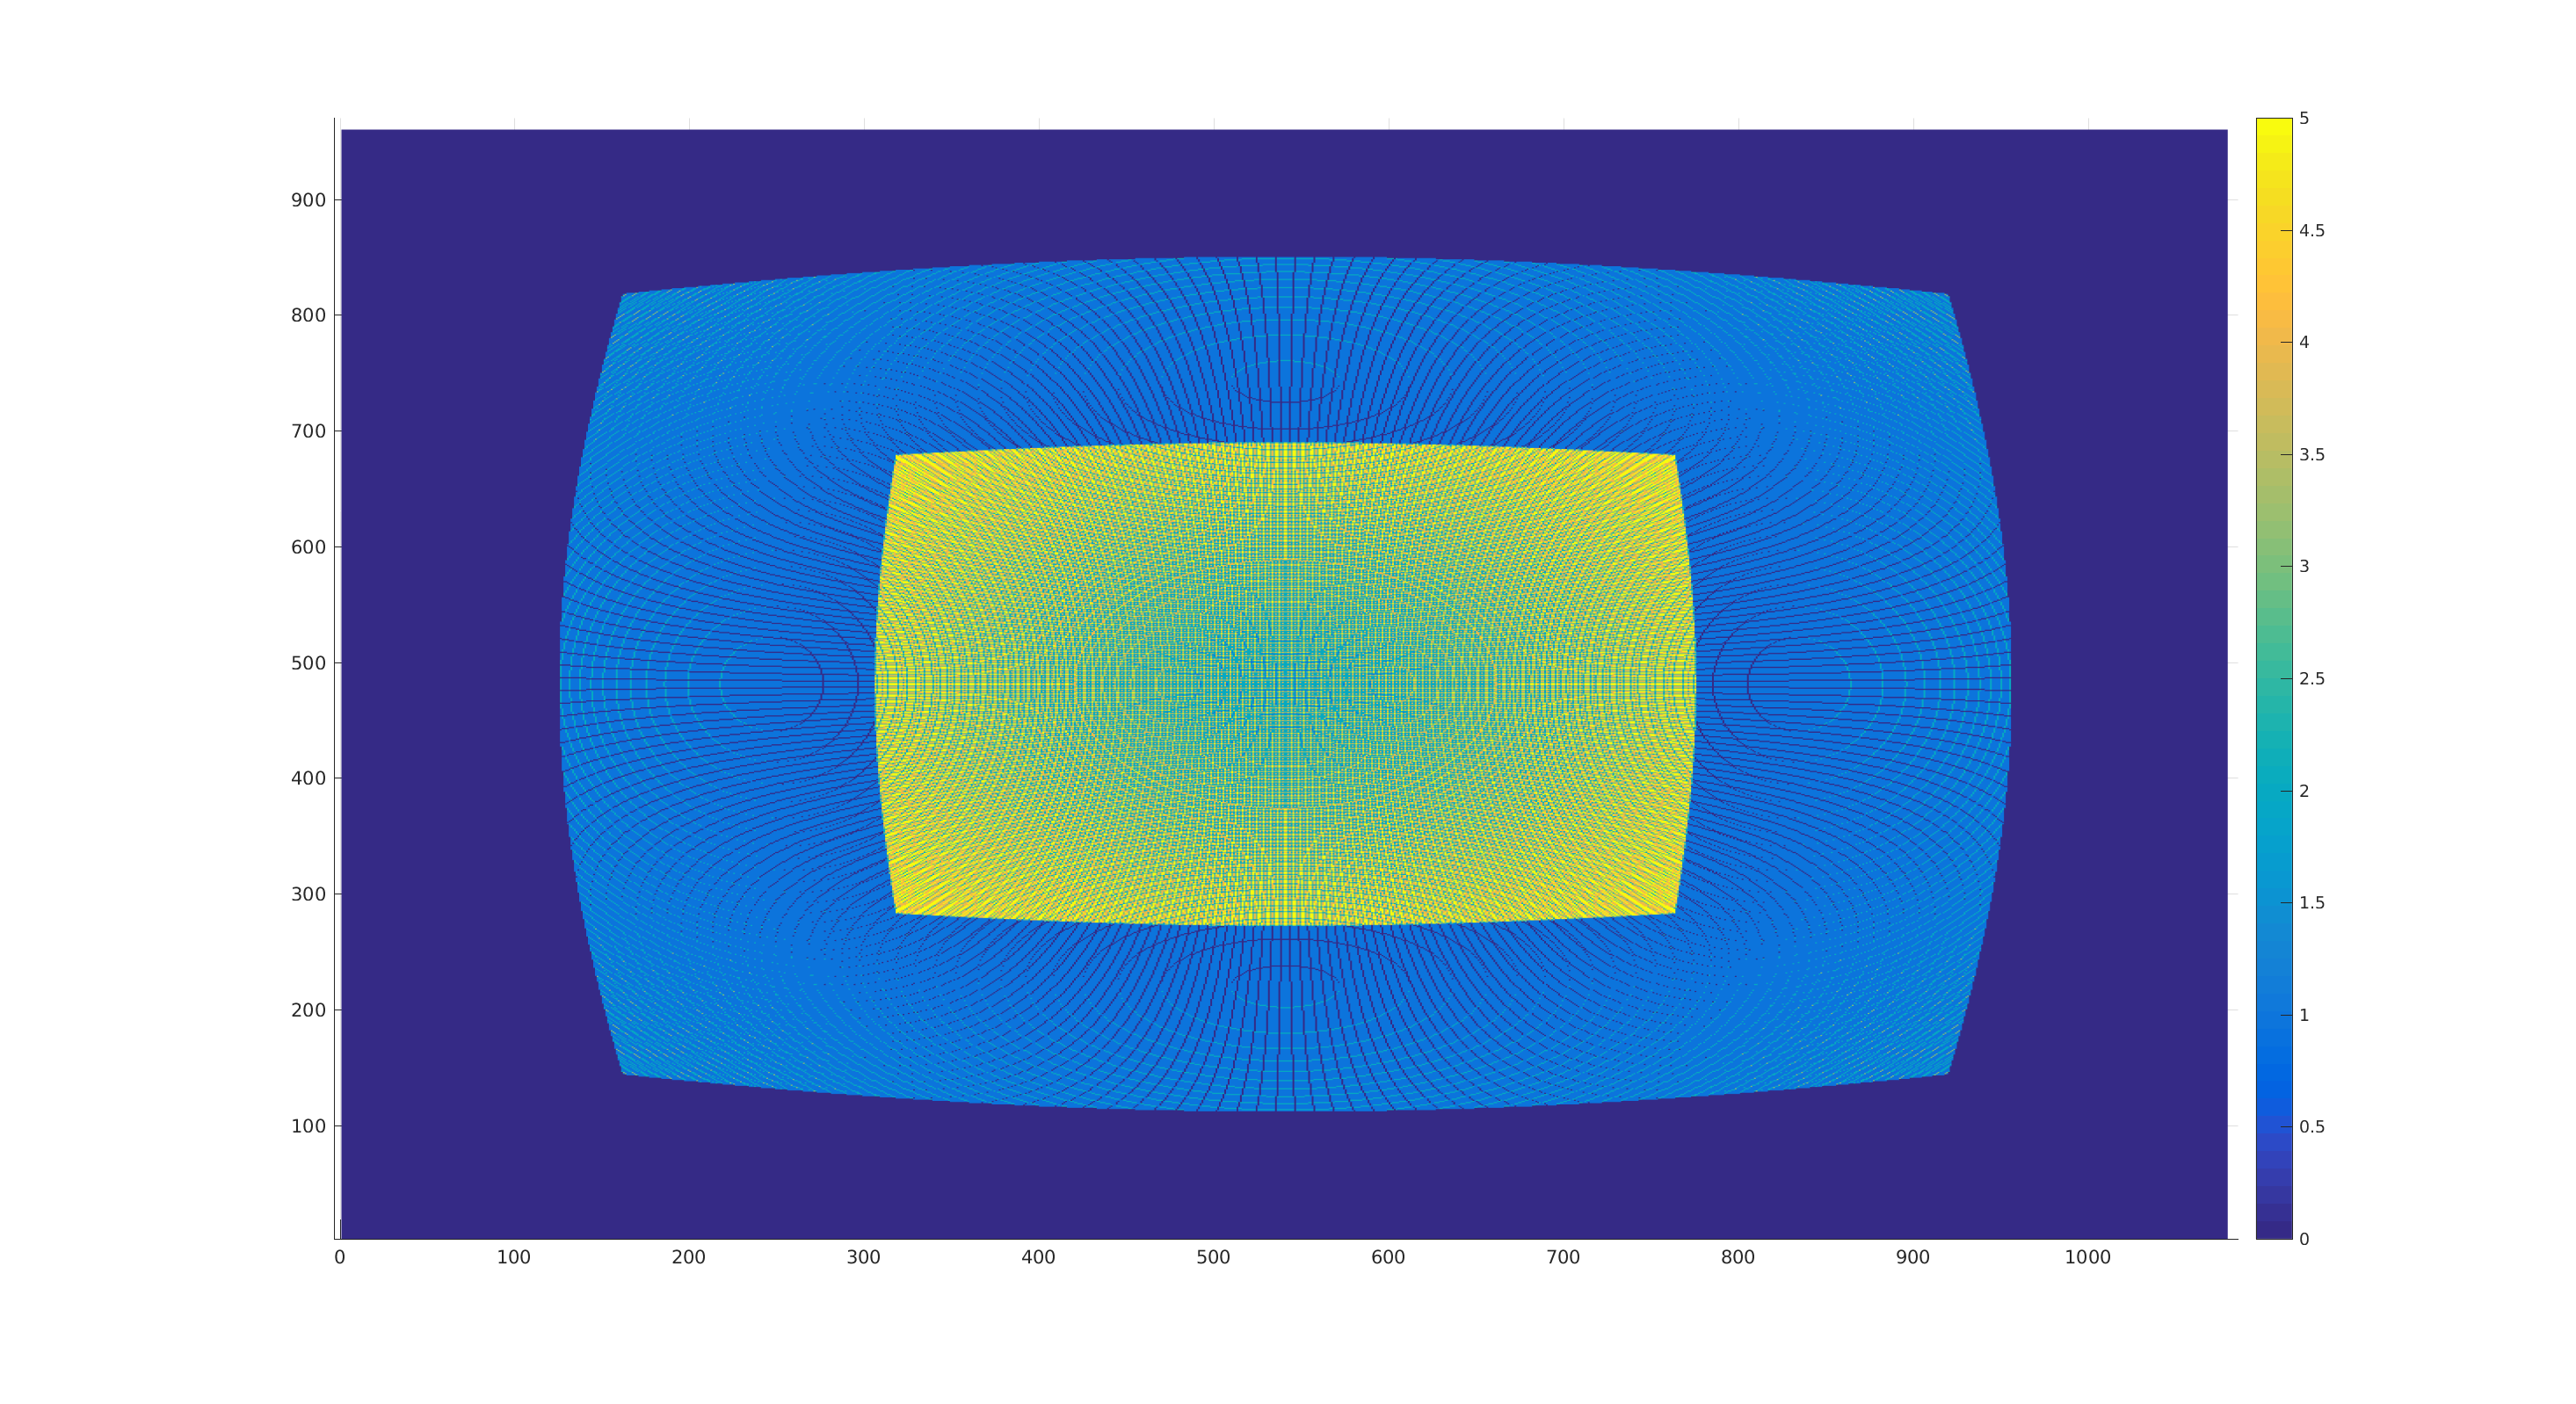
\includegraphics[width=1.2\linewidth]{figs/oculus_pixel_density_optimisation.eps}
\caption{Proposed texel density}
\label{epsfig1}
\end{subfigure}
 
\caption{Shows the texel to pixel density across a barrel distorted image.}
\label{fig:barreldensity}
\end{figure}

As can be seen by part B of figure \ref{fig:barreldensity}, by only rendering at full resolution in the center of the image, texel density is improved at the center, while decreasing the texel density in the edges of the image. The number of fragments that we shade is reduced by half, compared to the standard, non-supersampled image size that Oculus recommends. However, twice as many vertices need to be processed. Given that the bottleneck in most consumer applications are in the fragment shader stage, and that we generally need to process significantly more fragments that vertices, we should expect a considerable decrease in the time to present a frame using this method. 


\chapter{Conclusion}

This project's aim was to investigate common anti-aliasing techniques in the context of Virtual Reality. Two anti-aliasing techniques were developed and tested in a production demo, and one of these techniques was extended to perform more efficient stereoscopic rendering. As an extension, I modified one of these techniques to allow for texel density across the display to be efficiently increased at areas that are perceived as sharp, while decreasing it at blurrier areas. These techniques were profiled to assess their performance and image quality was assessed objectively.  

\section{Achievements}

All the implementations succeeded in shading fewer fragments than their respective usual implementations.
This shows promise where fragment shaders are becoming more complex and resolutions in Virtual Reality displays increase. \par

Though Subscreen Multisampling was almost indistinguishable from its fullscreen counterpart, implementation was not parallelisable because of limitations of the OpenGL API, and would be more inefficient for most applications. Though it would offer a speedup in applications where fragment processing is particularly time consuming.
Subscreen Supersampling was more visibly jarring, increased texture filtering in the center of the image along with noticeable alpha testing improvement meant that this technique was usually distinguishable from its fullscreen counterpart.
However, it's implementation shaded 49.5\% fewer fragments and was parallelisable allowing for processing time to be cut significantly. \par

The project extension allowed for 49.5\% fewer fragments to be shaded than standard rendering, while improving the texel density in the center of the image, where it is usually lowest and decreasing texel density at the edges where it is usually highest. The resolutions of both peripheral and central vision can be both tuned to achieve a more visually appealing result. - this does allow for fragment processing to be decreased significantly and gives a more texel density distribution that better represents the properties of the lenses. \par

These techniques were written to be applicable to any OpenGL forward renderer. They were first written in a toy renderer and then applied to a production demo.
While the method using the geometry shader is somewhat invasive to the vertex shader - I gave an example of future API functionality that can implement the same method, while being almost transparent to the vertex shader, and without the need of invoking the geometry shader stage.

\section{Final Remarks}

When asked about the performance gains Foveated Rendering would bring, John Carmark (Oculus CTO, Lead programmer of Doom, Quake) said: "Today, it might be a net negative due to rendering additional views. It will only be critical with much higher resolution displays.". In 2017, some GPU vendors have included multi-projection hardware allowing for multiple views to be rendered simultaneously, making this statement nearly obsolete - However, this multi-projection hardware is platform dependent. I gave a method for Multi-Projection in a platform independent setting, allowing for savings to be made in terms of fragment processing and frame render time.

%%%%%%%%%%%%%%%%%%%%%%%%%%%%%%%%%%%%%%%%%%%%%%%%%%%%%%%%%%%%%%%%%%%%%
% the bibliography
\addcontentsline{toc}{chapter}{Bibliography}
\bibliography{refs}

%%%%%%%%%%%%%%%%%%%%%%%%%%%%%%%%%%%%%%%%%%%%%%%%%%%%%%%%%%%%%%%%%%%%%
% the appendices
\appendix
\chapter{TODO}

\chapter{Project Proposal}

% Note: this file can be compiled on its own, but is also included by
% diss.tex (using the docmute.sty package to ignore the preamble)
\documentclass[12pt,a4paper,twoside]{article}
\usepackage[pdfborder={0 0 0}]{hyperref}
\usepackage[margin=25mm]{geometry}
\usepackage{graphicx}
\usepackage{parskip}
\begin{document}

\begin{center}
\Large
Computer Science Tripos -- Part II -- Project Proposal\\[4mm]
\LARGE
Smart Anti-Aliasing for Virtual Reality \\[4mm]

\large
G.~Ash, Fitzwilliam College

12 October 2016
\end{center}

\vspace{5mm}

\textbf{Project Supervisor:} Dr R.~Mantiuk

\textbf{Director of Studies:} Dr R.~Harle

\textbf{Project Overseers:} Prof R.~Anderson  \& Prof J.~Bacon

% Main document

\section*{Introduction}

A problem with modern Virtual Reality headsets is that they use low resolution displays to cover a huge Field of View.
Graphical artefacts, such as moir\'e patterns and pixellated edges (jaggies), are pronounced on these displays.
A good technique to ameliorate these artefacts if super-sampling, but super-sampling is often too expensive in VR
devices where low latency is a requirement - to avoid simulation sickness. 

Unfortunately, modern consumer headsets suffer from astigmatism because of a single lens between the viewer and the display. We can't remove these distortions without (another) anastigmatic lens, however we do currently give equal preference to image quality across the whole of the display even when the edges of the image become distorted.

\begin{figure}[tbh]
\centerline{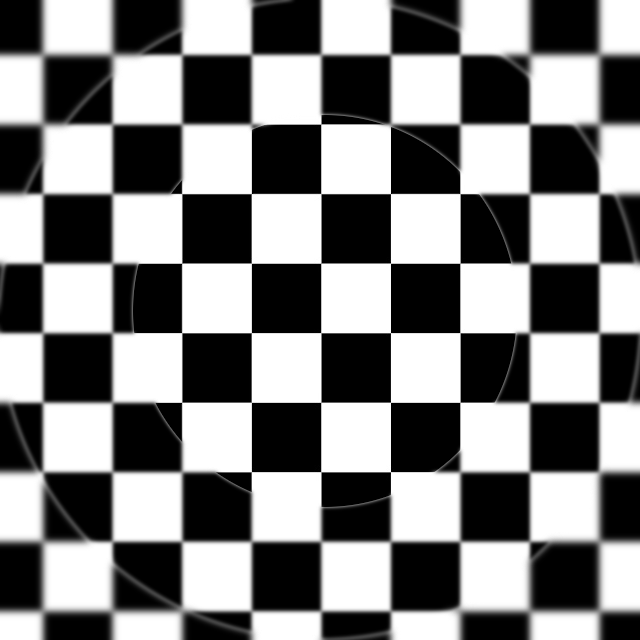
\includegraphics[width=0.3\linewidth]{figs/blur.png}}
\caption{The center of the perceived image is sharp, while the edges get progressively blurrier}
\label{blurfig}
\end{figure}

We could exploit astigmatism in single lens VR headsets by sampling more in the sharp center of the image,
and sampling less as we move towards the blurrier edges (Figure \ref{blurfig}). This project aims to extend an existing open source system to include this optimisation, and to measure the impact on both the performance of the system, and on the image quality to the user.

\section*{Starting point}

Novel anti-aliasing techniques, such as subpixel-reconstruction and temporal antialiasing, are still actively being developed. I intend to build on Intel's research[1] into a hybrid raytracing/rasterizing VR renderer by creating an entirely rasterized solution that retains image quality while allowing for GPU hardware acceleration.

Free and extensible renderers exist for VR headsets, such as Unity. However I will be extending the existing open-source OSVR-RenderManager, which will allow me to easily create separate reusable demos to show off certain graphical artefacts, and, if neccesary, to modify the entire rendering pipeline.
OSVR is compatible with all modern VR headsets, and supports all modern graphics APIs (OpenGL, Vulkan, Direct3D).

I have good experience in C/C++ through small projects and the IB C/C++ course. I'm familiar with the graphics pipeline and have experience in WebGL, with some experience writing vertex and fragment shaders in OpenGL. I will need to refresh my knowledge of shader programming, and will need to take some time learning most of the OpenGL API.

\section*{Resources required}

For this project I shall be using my own quad-core machine with a VR capable GPU. I will also be using an Occulus Rift Development Kit 2 [3](lent to me by the Hackers at Cambridge group) for testing and user studies. Source backups will be made both to a private Github repository and MCS daily.
I will use an MCS machine as a failsafe incase my machine should break.

\section*{Work to be done}

The project breaks down into the following sub-projects:

\begin{enumerate}

\item \textbf{Setup} Fork the existing Open Source Virtual Reality-RenderManager repository. Create a daily cronjob to backup this to github and MCS. Research my chosen renderer's pipeline.

\item \textbf {Core development} Develop/modify a simple super-sampling algorithm. Extend the algorithm to allow for areas of the screen to be ignored. Further extend to seamlessly composite draws that we sample differently.

\item \textbf {Demo creation} Create a couple of OpenGL demos that highlight both moire patterns and pixellated edges, for use in visual quality experiment.

\item \textbf {Optimisation} Make use of a GPU profiler to determine any redundancy or inefficiency. Refactor the algorithm to make it easily configurable.

\item \textbf {Evaluation} Make use of benchmarking/profiling software to evaluate the algorithm with regards to performance. Perform visual quality experiment to evaluate the impact of the algorithm on image quality to the user, recruit college members across fields to participate. Compare my approach against no anti-aliasing, and fullscreen anti-aliasing.

\end{enumerate}

\section*{Success citeria}

The project will be a success if I manage to do the following:
\begin{enumerate}

\item Improve the performance of the open source renderer with anti-aliasing enabled

\item Provide an alternative anti-aliasing technique that suffers only negligible loss in image quality to the end user.

\item Evaluate both full screen antialiasing, my selective antialiasing approach, and no antialiasing from a user perspective by constructing demos that show off artefacts masked by antialiasing.

\end{enumerate}

\section*{Possible extensions}

If I achieve my main result early I shall try the following
alternative experiment or method of evaluation:

\begin{enumerate}

\item Research using a heuristic to determine salient objects or regions in the scene, and extend my algorithm to more closely resemble a foveated rendering[2] technique.

\item Further reduce the requirement to super-sample by determining which objects/samples can be shared between each eye.

\end{enumerate}





\section*{Timetable}

Planned starting date is 16/10/2011.

\begin{enumerate}

\item \textbf{Michaelmas weeks 2--4} Start project Setup, Begin refreshing knowledge on OpenGL. Research the rendering pipeline of my chosen renderer. Formulate an implementation strategy.

\item \textbf{Michaelmas weeks 5--6} Complete project setup. Test writing custom code in the renderer, start implementation of selective antialiasing algorithm

\item \textbf{Michaelmas weeks 7--8} Continue development of algorithm. Start on demo creation

\item \textbf{Michaelmas vacation} Finish development of algorithm and demos.

\item \textbf{Lent weeks 0--2} Write progress report. Generate corpus of
  test examples. Begin optimisation.

\item \textbf{Lent weeks 3--5} Finish optimisation, begin evaluation of image quality on users.  

\item \textbf{Lent weeks 6--8} Finish user studies, start performance analysis. Write up User studies in disseration.

\item \textbf{Easter vacation:} Begin on extensions, flesh out dissertation, complete evaluation. 

\item \textbf{Easter term 0--2:}  Complete dissertation, proof read. Submit to DoS and supervisor for comments. 

\item \textbf{Easter term 3:} Further proof reading/refactoring and submit dissertation.

\end{enumerate}

\section*{References}

\begin{enumerate}

\item Using Astigmatism in Wide Angle HMDs to Improve Rendering D. Pohl, T. Bolkart, S. Nickels, O. Grau, 2015.
\item Foveated 3d graphics. B. Guenter, M. Finch, S. Drucker, D. Tan, and J. Snyder. ACM SIGGRAPH Asia, 2012.
\item Oculus VR. Oculus Rift, 2014. http://www.oculus.com/

\end{enumerate}

\end{document}


\end{document}
